%%%% Proceedings format for most of ACM conferences (with the exceptions listed below) and all ICPS volumes.

\documentclass[sigplan,10pt, review]{acmart}\settopmatter{printfolios=true,printccs=false,printacmref=false}

%\documentclass[sigconf]{acmart}

\usepackage{booktabs} % For formal tables
\usepackage{amsmath}
\usepackage{amssymb}
\usepackage{stmaryrd}
\usepackage{mathtools}
\usepackage[ruled]{algorithm2e} % For algorithms
\usepackage{listings}
\usepackage{subfig}

\newcommand{\todo}{\textcolor{red}{\textbf{TODO}}}
\newcommand{\var}[1]{\mathit{#1}}
\newcommand{\bv}[1]{#1~\mathit{word}}
\newcommand{\bitmoded}[2]{{\underbracket[1pt][1pt]{#2}_{#1}}}
\newcommand{\bitmodeu}[2]{{\overbracket[1pt][1pt]{#2}^{#1}}}
\newcommand{\testbit}{~!!~}
\newcommand{\nocompile}[1]{}
\newcommand{\CC}{C\nolinebreak\hspace{-.05em}\raisebox{.4ex}{\small +}\nolinebreak\hspace{-.10em}\raisebox{.4ex}{\small +}}

\DeclareMathOperator{\ucast}{zxtend}
\DeclareMathOperator{\sint}{sint}
\DeclareMathOperator{\msb}{msb}
\DeclareMathOperator{\sextend}{sxtend}
\DeclareMathOperator{\zextend}{zxtend}
\DeclareMathOperator{\rev}{rev}
\DeclareMathOperator{\bytesof}{bytes\_of}
\DeclareMathOperator{\parity}{parity}
\DeclareMathOperator{\fold}{fold}
\DeclareMathOperator{\sign}{sign}
\DeclareMathOperator{\isNaN}{isNaN}

\renewcommand{\algorithmcfname}{ALGORITHM}
\SetAlFnt{\small}
\SetAlCapFnt{\small}
\SetAlCapNameFnt{\small}
\SetAlCapHSkip{0pt}
\IncMargin{-\parindent}

\lstdefinestyle{customc}{
  language=C,
  basicstyle=\small
}

\lstdefinelanguage
   [x64]{Assembler}     % add a "x64" dialect of Assembler
   [x86masm]{Assembler} % based on the "x86masm" dialect
   % with these extra keywords:
   {morekeywords={CDQE,CQO,CMPSQ,CMPXCHG16B,JRCXZ,LODSQ,MOVSXD, %
                  POPFQ,PUSHFQ,SCASQ,STOSQ,IRETQ,RDTSCP,SWAPGS, %
                  rax,rdx,rcx,rbx,rsi,rdi,rsp,rbp, %
                  r8,r8d,r8w,r8b,r9,r9d,r9w,r9b, %
                  r10,r10d,r10w,r10b,r11,r11d,r11w,r11b, %
                  r12,r12d,r12w,r12b,r13,r13d,r13w,r13b, %
                  r14,r14d,r14w,r14b,r15,r15d,r15w,r15b}} % etc.

\lstdefinestyle{customasm}{
  belowcaptionskip=1\baselineskip,
  language=[x64]Assembler,
  basicstyle=\ttfamily,
	keywordstyle=\ttfamily,
  commentstyle=\itshape,
}

\lstset{escapeinside={(*@}{@*)},language=[x64]Assembler,style=customasm,morecomment=[l][\itshape]{\#}}


% Copyright
 \setcopyright{none}
%\setcopyright{acmcopyright}
%\setcopyright{acmlicensed}
%\setcopyright{rightsretained}
%\setcopyright{usgov}
%\setcopyright{usgovmixed}
%\setcopyright{cagov}
%\setcopyright{cagovmixed}

% DOI
\acmDOI{}
\acmISBN{}

%Conference
\acmConference[CPP'19]{ACM SIGPLAN International Conference on Certified Programs and Proofs}{January 2019}{Lisbon, Portugal}
\acmYear{2019}
\startPage{1}

\begin{document}
% Title portion. Note the short title for running heads
\title{Formally Verified Big Step Semantics out of x86-64 Binaries}

\author{Ian Roessle}
%\orcid{1234-5678-9012-3456}
\affiliation{%
  \institution{Virginia Polytechnic Institute and State University}
  \streetaddress{}
  \city{}
  \state{}
  \postcode{}
  \country{}
}
\email{iroessle@vt.edu}
\author{Freek Verbeek}
\affiliation{%
  \institution{Virginia Polytechnic Institute and State University}
  \streetaddress{}
  \city{}
  \state{}
  \postcode{}
  \country{}
}
\email{freek@vt.edu}
\author{Binoy Ravindran}
\affiliation{%
  \institution{Virginia Polytechnic Institute and State University}
  \streetaddress{}
  \city{}
  \state{}
  \postcode{}
  \country{}
}
\email{binoy@vt.edu}


\begin{abstract}
This paper presents a methodology for generating formally proven equivalence theorems between decompiled x86-64 machine code and big step semantics. 
These proofs are built on top of two additional contributions. 
First, a robust and tested formal x86-64 machine model containing small step semantics for 1625 instructions.
Second, a decompilation-into-logic methodology supporting both x86-64 assembly and machine code at large scale.
This work enables black-box binary verification, i.e., formal verification of a binary where source code is unavailable.
As such, it can be applied to safety-critical systems that consist of legacy components, or components whose source code is unavailable due to proprietary reasons.
The methodology minimizes the trusted code base by leveraging machine-learned semantics to build a formal machine model.
We apply the methodology to several case studies, including binaries that heavily rely on the SSE2 floating-point instruction set, and binaries that are obtained by compiling code that is obtained by inlining assembly into C code.
%Between the optimization of compiliers and a lack of formal instruction semantics, lifting x86-64 binaries and formaly verifying them to a specification has been fraught with difficulty. As such, most formal verification methodologies often operate at a higher level of abstraction to the binary and rely on trusted compilers. Operating systems often however leverage custom assembly or a hybrid of C++ and Assembly in order for performance, which would would not work with former approaches. Leviathan's main contribution is a step toward enabling verification at the binary level -- namely that of lifting an x86-64 binary up to big step semantics for formal verification at a more abstrat level of representation.
\end{abstract}



%
% The code below should be generated by the tool at
% http://dl.acm.org/ccs.cfm
% Please copy and paste the code instead of the example below.
%
\begin{CCSXML}

<concept>
<concept_id>10003752.10003790.10003798</concept_id>
 <concept_desc>Theory of computation~Equational logic and rewriting</concept_desc>
<concept_significance>500</concept_significance>
</concept>

<concept>
<concept_id>10003752.10003790.10011119</concept_id>
 <concept_desc>Theory of computation~Abstraction</concept_desc>
<concept_significance>500</concept_significance>
</concept>
</ccs2012>


\end{CCSXML}

 \ccsdesc[500]{Theory of computation~Equational logic and rewriting}
 \ccsdesc[500]{Theory of computation~Abstraction}

 %
% End generated code
%


\keywords{x86-64,
semantics, theorem proving}


\maketitle


% The default list of authors is too long for headers.
\renewcommand{\shortauthors}{I. Roessle et al.}


%\section{Introduction}

The \textit{proceedings} are the records of a conference.\footnote{This
  is a footnote}  ACM seeks
to give these conference by-products a uniform, high-quality
appearance.  To do this, ACM has some rigid requirements for the
format of the proceedings documents: there is a specified format
(balanced double columns), a specified set of fonts (Arial or
Helvetica and Times Roman) in certain specified sizes, a specified
live area, centered on the page, specified size of margins, specified
column width and gutter size.

\section{The Body of The Paper}
Typically, the body of a paper is organized into a hierarchical
structure, with numbered or unnumbered headings for sections,
subsections, sub-subsections, and even smaller sections.  The command
\texttt{{\char'134}section} that precedes this paragraph is part of
such a hierarchy.\footnote{This is a footnote.} \LaTeX\ handles the
numbering and placement of these headings for you, when you use the
appropriate heading commands around the titles of the headings.  If
you want a sub-subsection or smaller part to be unnumbered in your
output, simply append an asterisk to the command name.  Examples of
both numbered and unnumbered headings will appear throughout the
balance of this sample document.

Because the entire article is contained in the \textbf{document}
environment, you can indicate the start of a new paragraph with a
blank line in your input file; that is why this sentence forms a
separate paragraph.

\subsection{Type Changes and {\itshape Special} Characters}

We have already seen several typeface changes in this sample.  You can
indicate italicized words or phrases in your text with the command
\texttt{{\char'134}textit}; emboldening with the command
\texttt{{\char'134}textbf} and typewriter-style (for instance, for
computer code) with \texttt{{\char'134}texttt}.  But remember, you do
not have to indicate typestyle changes when such changes are part of
the \textit{structural} elements of your article; for instance, the
heading of this subsection will be in a sans serif\footnote{Another
  footnote here.  Let's make this a rather long one to see how it
  looks.} typeface, but that is handled by the document class file.
Take care with the use of\footnote{Another footnote.}  the
curly braces in typeface changes; they mark the beginning and end of
the text that is to be in the different typeface.

You can use whatever symbols, accented characters, or non-English
characters you need anywhere in your document; you can find a complete
list of what is available in the \textit{\LaTeX\ User's Guide}
\cite{Lamport:LaTeX}.

\subsection{Math Equations}
You may want to display math equations in three distinct styles:
inline, numbered or non-numbered display.  Each of
the three are discussed in the next sections.

\subsubsection{Inline (In-text) Equations}
A formula that appears in the running text is called an
inline or in-text formula.  It is produced by the
\textbf{math} environment, which can be
invoked with the usual \texttt{{\char'134}begin\,\ldots{\char'134}end}
construction or with the short form \texttt{\$\,\ldots\$}. You
can use any of the symbols and structures,
from $\alpha$ to $\omega$, available in
\LaTeX~\cite{Lamport:LaTeX}; this section will simply show a
few examples of in-text equations in context. Notice how
this equation:
\begin{math}
  \lim_{n\rightarrow \infty}x=0
\end{math},
set here in in-line math style, looks slightly different when
set in display style.  (See next section).

\subsubsection{Display Equations}
A numbered display equation---one set off by vertical space from the
text and centered horizontally---is produced by the \textbf{equation}
environment. An unnumbered display equation is produced by the
\textbf{displaymath} environment.

Again, in either environment, you can use any of the symbols
and structures available in \LaTeX\@; this section will just
give a couple of examples of display equations in context.
First, consider the equation, shown as an inline equation above:
\begin{equation}
  \lim_{n\rightarrow \infty}x=0
\end{equation}
Notice how it is formatted somewhat differently in
the \textbf{displaymath}
environment.  Now, we'll enter an unnumbered equation:
\begin{displaymath}
  \sum_{i=0}^{\infty} x + 1
\end{displaymath}
and follow it with another numbered equation:
\begin{equation}
  \sum_{i=0}^{\infty}x_i=\int_{0}^{\pi+2} f
\end{equation}
just to demonstrate \LaTeX's able handling of numbering.

\subsection{Citations}
Citations to articles~\cite{bowman:reasoning,
clark:pct, braams:babel, herlihy:methodology},
conference proceedings~\cite{clark:pct} or maybe
books \cite{Lamport:LaTeX, salas:calculus} listed
in the Bibliography section of your
article will occur throughout the text of your article.
You should use BibTeX to automatically produce this bibliography;
you simply need to insert one of several citation commands with
a key of the item cited in the proper location in
the \texttt{.tex} file~\cite{Lamport:LaTeX}.
The key is a short reference you invent to uniquely
identify each work; in this sample document, the key is
the first author's surname and a
word from the title.  This identifying key is included
with each item in the \texttt{.bib} file for your article.

The details of the construction of the \texttt{.bib} file
are beyond the scope of this sample document, but more
information can be found in the \textit{Author's Guide},
and exhaustive details in the \textit{\LaTeX\ User's
Guide} by Lamport~\shortcite{Lamport:LaTeX}.

This article shows only the plainest form
of the citation command, using \texttt{{\char'134}cite}.

Some examples.  A paginated journal article \cite{Abril07}, an enumerated
journal article \cite{Cohen07}, a reference to an entire issue \cite{JCohen96},
a monograph (whole book) \cite{Kosiur01}, a monograph/whole book in a series (see 2a in spec. document)
\cite{Harel79}, a divisible-book such as an anthology or compilation \cite{Editor00}
followed by the same example, however we only output the series if the volume number is given
\cite{Editor00a} (so Editor00a's series should NOT be present since it has no vol. no.),
a chapter in a divisible book \cite{Spector90}, a chapter in a divisible book
in a series \cite{Douglass98}, a multi-volume work as book \cite{Knuth97},
an article in a proceedings (of a conference, symposium, workshop for example)
(paginated proceedings article) \cite{Andler79}, a proceedings article
with all possible elements \cite{Smith10}, an example of an enumerated
proceedings article \cite{VanGundy07},
an informally published work \cite{Harel78}, a doctoral dissertation \cite{Clarkson85},
a master's thesis: \cite{anisi03}, an online document / world wide web
resource \cite{Thornburg01, Ablamowicz07, Poker06}, a video game (Case 1) \cite{Obama08} and (Case 2) \cite{Novak03}
and \cite{Lee05} and (Case 3) a patent \cite{JoeScientist001},
work accepted for publication \cite{rous08}, 'YYYYb'-test for prolific author
\cite{SaeediMEJ10} and \cite{SaeediJETC10}. Other cites might contain
'duplicate' DOI and URLs (some SIAM articles) \cite{Kirschmer:2010:AEI:1958016.1958018}.
Boris / Barbara Beeton: multi-volume works as books
\cite{MR781536} and \cite{MR781537}.

A couple of citations with DOIs: \cite{2004:ITE:1009386.1010128,
  Kirschmer:2010:AEI:1958016.1958018}.

Online citations: \cite{TUGInstmem, Thornburg01, CTANacmart}.


\subsection{Tables}
Because tables cannot be split across pages, the best
placement for them is typically the top of the page
nearest their initial cite.  To
ensure this proper ``floating'' placement of tables, use the
environment \textbf{table} to enclose the table's contents and
the table caption.  The contents of the table itself must go
in the \textbf{tabular} environment, to
be aligned properly in rows and columns, with the desired
horizontal and vertical rules.  Again, detailed instructions
on \textbf{tabular} material
are found in the \textit{\LaTeX\ User's Guide}.

Immediately following this sentence is the point at which
Table~\ref{tab:freq} is included in the input file; compare the
placement of the table here with the table in the printed
output of this document.

\begin{table}
  \caption{Frequency of Special Characters}
  \label{tab:freq}
  \begin{tabular}{ccl}
    \toprule
    Non-English or Math&Frequency&Comments\\
    \midrule
    \O & 1 in 1,000& For Swedish names\\
    $\pi$ & 1 in 5& Common in math\\
    \$ & 4 in 5 & Used in business\\
    $\Psi^2_1$ & 1 in 40,000& Unexplained usage\\
  \bottomrule
\end{tabular}
\end{table}

To set a wider table, which takes up the whole width of the page's
live area, use the environment \textbf{table*} to enclose the table's
contents and the table caption.  As with a single-column table, this
wide table will ``float'' to a location deemed more desirable.
Immediately following this sentence is the point at which
Table~\ref{tab:commands} is included in the input file; again, it is
instructive to compare the placement of the table here with the table
in the printed output of this document.


\begin{table*}
  \caption{Some Typical Commands}
  \label{tab:commands}
  \begin{tabular}{ccl}
    \toprule
    Command &A Number & Comments\\
    \midrule
    \texttt{{\char'134}author} & 100& Author \\
    \texttt{{\char'134}table}& 300 & For tables\\
    \texttt{{\char'134}table*}& 400& For wider tables\\
    \bottomrule
  \end{tabular}
\end{table*}
% end the environment with {table*}, NOTE not {table}!

It is strongly recommended to use the package booktabs~\cite{Fear05}
and follow its main principles of typography with respect to tables:
\begin{enumerate}
\item Never, ever use vertical rules.
\item Never use double rules.
\end{enumerate}
It is also a good idea not to overuse horizontal rules.


\subsection{Figures}

Like tables, figures cannot be split across pages; the best placement
for them is typically the top or the bottom of the page nearest their
initial cite.  To ensure this proper ``floating'' placement of
figures, use the environment \textbf{figure} to enclose the figure and
its caption.

This sample document contains examples of \texttt{.eps} files to be
displayable with \LaTeX.  If you work with pdf\LaTeX, use files in the
\texttt{.pdf} format.  Note that most modern \TeX\ systems will convert
\texttt{.eps} to \texttt{.pdf} for you on the fly.  More details on
each of these are found in the \textit{Author's Guide}.

\begin{figure}

\includegraphics{fly}
\caption{A sample black and white graphic.}
\end{figure}

\begin{figure}

\includegraphics[height=1in, width=1in]{fly}
\caption{A sample black and white graphic
that has been resized with the \texttt{includegraphics} command.}
\end{figure}


As was the case with tables, you may want a figure that spans two
columns.  To do this, and still to ensure proper ``floating''
placement of tables, use the environment \textbf{figure*} to enclose
the figure and its caption.  And don't forget to end the environment
with \textbf{figure*}, not \textbf{figure}!

\begin{figure*}
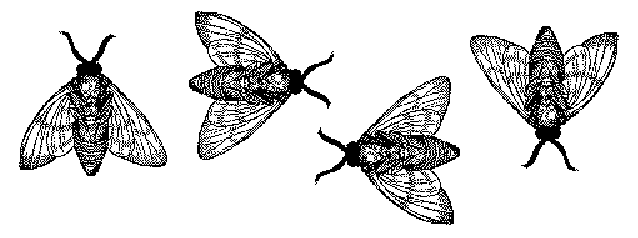
\includegraphics{flies}
\caption{A sample black and white graphic
that needs to span two columns of text.}
\end{figure*}


\begin{figure}

\includegraphics[height=1in, width=1in]{rosette}
\caption{A sample black and white graphic that has
been resized with the \texttt{includegraphics} command.}
\end{figure}

\subsection{Theorem-like Constructs}

Other common constructs that may occur in your article are the forms
for logical constructs like theorems, axioms, corollaries and proofs.
ACM uses two types of these constructs:  theorem-like and
definition-like.

Here is a theorem:
\begin{theorem}
  Let $f$ be continuous on $[a,b]$.  If $G$ is
  an antiderivative for $f$ on $[a,b]$, then
  \begin{displaymath}
    \int^b_af(t)\,dt = G(b) - G(a).
  \end{displaymath}
\end{theorem}

Here is a definition:
\begin{definition}
  If $z$ is irrational, then by $e^z$ we mean the
  unique number that has
  logarithm $z$:
  \begin{displaymath}
    \log e^z = z.
  \end{displaymath}
\end{definition}

The pre-defined theorem-like constructs are \textbf{theorem},
\textbf{conjecture}, \textbf{proposition}, \textbf{lemma} and
\textbf{corollary}.  The pre-defined de\-fi\-ni\-ti\-on-like constructs are
\textbf{example} and \textbf{definition}.  You can add your own
constructs using the \textsl{amsthm} interface~\cite{Amsthm15}.  The
styles used in the \verb|\theoremstyle| command are \textbf{acmplain}
and \textbf{acmdefinition}.

Another construct is \textbf{proof}, for example,

\begin{proof}
  Suppose on the contrary there exists a real number $L$ such that
  \begin{displaymath}
    \lim_{x\rightarrow\infty} \frac{f(x)}{g(x)} = L.
  \end{displaymath}
  Then
  \begin{displaymath}
    l=\lim_{x\rightarrow c} f(x)
    = \lim_{x\rightarrow c}
    \left[ g{x} \cdot \frac{f(x)}{g(x)} \right ]
    = \lim_{x\rightarrow c} g(x) \cdot \lim_{x\rightarrow c}
    \frac{f(x)}{g(x)} = 0\cdot L = 0,
  \end{displaymath}
  which contradicts our assumption that $l\neq 0$.
\end{proof}

\section{Conclusions}
This paragraph will end the body of this sample document.
Remember that you might still have Acknowledgments or
Appendices; brief samples of these
follow.  There is still the Bibliography to deal with; and
we will make a disclaimer about that here: with the exception
of the reference to the \LaTeX\ book, the citations in
this paper are to articles which have nothing to
do with the present subject and are used as
examples only.
%\end{document}  % This is where a 'short' article might terminate



\appendix
%Appendix A
\section{Headings in Appendices}
The rules about hierarchical headings discussed above for
the body of the article are different in the appendices.
In the \textbf{appendix} environment, the command
\textbf{section} is used to
indicate the start of each Appendix, with alphabetic order
designation (i.e., the first is A, the second B, etc.) and
a title (if you include one).  So, if you need
hierarchical structure
\textit{within} an Appendix, start with \textbf{subsection} as the
highest level. Here is an outline of the body of this
document in Appendix-appropriate form:
\subsection{Introduction}
\subsection{The Body of the Paper}
\subsubsection{Type Changes and  Special Characters}
\subsubsection{Math Equations}
\paragraph{Inline (In-text) Equations}
\paragraph{Display Equations}
\subsubsection{Citations}
\subsubsection{Tables}
\subsubsection{Figures}
\subsubsection{Theorem-like Constructs}
\subsubsection*{A Caveat for the \TeX\ Expert}
\subsection{Conclusions}
\subsection{References}
Generated by bibtex from your \texttt{.bib} file.  Run latex,
then bibtex, then latex twice (to resolve references)
to create the \texttt{.bbl} file.  Insert that \texttt{.bbl}
file into the \texttt{.tex} source file and comment out
the command \texttt{{\char'134}thebibliography}.
% This next section command marks the start of
% Appendix B, and does not continue the present hierarchy
\section{More Help for the Hardy}

Of course, reading the source code is always useful.  The file
\path{acmart.pdf} contains both the user guide and the commented
code.

\begin{acks}
  The authors would like to thank Dr. Yuhua Li for providing the
  MATLAB code of the \textit{BEPS} method.

  The authors would also like to thank the anonymous referees for
  their valuable comments and helpful suggestions. The work is
  supported by the \grantsponsor{GS501100001809}{National Natural
    Science Foundation of
    China}{http://dx.doi.org/10.13039/501100001809} under Grant
  No.:~\grantnum{GS501100001809}{61273304}
  and~\grantnum[http://www.nnsf.cn/youngscientists]{GS501100001809}{Young
    Scientists' Support Program}.

\end{acks}

% Head 1


\section{Introduction}

%\\
%\\

This paper targets bottom-up formal verification, i.e., verification of binaries where source code is unavailable.
Our aim is to use formal methods to analyze legacy systems, or systems where source code is unavailable due to proprietary reasons.
Various safety-critical systems in automotive, aerospace, medical and military domains are built out of components where the source code is not available~\cite{sulaman2014development}.
In such a context, certification plays a crucial role.
Certification can require a compliance proof based on formal methods~\cite{rushby1997formal,Woodcock09}.
Bottom-up formal verification can aid in obtaining high levels of assurance for black-box components running on commodity hardware, such as x86-64.

A binary typically consists of \emph{blocks} composed by \emph{control flow}.
In this paper, a block is defined as a sequence of instructions that can be modeled with only if-then-else statements (no loops).
A formal model of a binary can be obtained by translating, e.g., loops to recursive functions, and blocks to sequences of state updates.
Each state update corresponds to the semantics of one instruction, dictated by a \emph{machine model}.
We call this the \emph{small-step semantics} of that block.
This approach is called \emph{decompilation-into-logic} (DiL)~\cite{4689183,myreen2012decompilation}.
The model obtained by DiL can, e.g., then be used to prove correspondence to source code.

In a context where source code is unavailable, however, small-step semantics do not suffice.
A block can consist of dozens of lines of machine code that is unintelligible and not suitable for further analysis.
This paper presents a methodology that largely automatically derives a formal model for a block in a binary that is on the same level of abstraction as C.
We call this the \emph{big-step semantics} of that block.
This provides insight into the semantics of the binary and enables use of the generated formal model for correctness proofs.
Moreover, it provides a user with insight into the branching conditions in the binary, which can aid in building test suites.

% TCB
%Of particular note within any formal verification effort is the TCB~\cite{kumarsoftware}.
%Determining the exact semantics of the many x86-64 instructions is hard: even the Intel manual describing them may contain errors.
%Hand-writing a machine model of the x86-64 architecture would add thousands of lines of unreliable code to the TCB.
%We therefore utilize the machine learned semantics of Heule et al.~\cite{heule2016}.
%We present a way of embedding these semantics into HOL, producing a highly reliable formal x86-64 machine model
%To increase reliability, we automatically prove millions of test lemma's, testing the machine model against running binaries on an x86-64 machine.

Of particular note within any formal verification effort is the trusted code base (TCB)~\cite{kumarsoftware}.
Specifically, the machine model is part of the TCB.
The x86-64 architecture presents a unique challenge, due to the lack of a formal specification.
%This creates an inherent inference problem with respect to what the actual architecture specification is.
Hand-writing a machine model of the x86-64 architecture is inherently based on semi-formal Intel manuals. 
Therefore, Heule et al. applied machine learning to \emph{infer} semantics from live x86-64 hardware~\cite{heule2016}.
Their approach produced semantics that are more reliable than the Intel manuals.
We provide a DiL framework that maps instructions in a binary to machine learned semantics.
%In contrast, we utilize the machine learned semantics of Heule et al.~\cite{heule2016}.
This has an additional advantage that it learns a set of test cases that cover intricate corner cases.
We automatically prove millions of lemmas using these test cases, which validate our machine model against live x86-64 hardware.

This paper presents the following contributions: 1.) a largely automated way to generate big-step semantics of blocks in a binary, plus a formal proof of equivalence between big- and small-step semantics, based on 2.) a machine learned and formally tested x86-64 machine model containing 1625 IVs, and 3.) a re-implementation of decompilation-into-logic for x86-64 and the Isabelle/HOL theorem prover~\cite{nipkow2002isabelle,dawson2009isabelle}.
The latter applies to both machine code and assembly, making it possible to leverage recent advances in \emph{reassembly}~\cite{wang2017ramblr}.

% Limitations
The challenge of binary verification is the semantical gap between a source language and a binary.
This introduces some limitations.
Specifically, we are not able to extract typing information.
Local variables and values in memory have a known size, but their type is unknown.
Our machine model does not deal with concurrency.
We cannot deal with self-modifying code.
To support calls to library functions and indirect calls, a more advanced memory model is needed, allowing assumptions on where loaded libraries are stored.
Finally, we have targeted x86-64 specifically, instead of making the methodology generic.


% RESULTS: various small examples + one (?) case study
The methodology is applied to several examples to show that it is able to deal with, e.g., if-then-else structures, floating-point operations and pointers.
We verify an example where the binary has been obtained by compiling C code mixed with inline assembly.
%We also verified an example written in \CC, even though we had no formal semantics of that language.
We also verify a binary containing the remainder function from the FDLIBM floating point library\footnote{\url{http://www.netlib.org/fdlibm/}}.
For each case study, we show that the big-step semantics lifted out of the binary is a close match to the original source code.
All case studies and the Isabelle/HOL proofs are publicly available at: \url{https://filebox.ece.vt.edu/~iroessle/cpp\_2019.zip}

% OUTRO
The next section presents an overview of our methodology, and the structure of this paper.

\section{Methodology}

\begin{figure*}
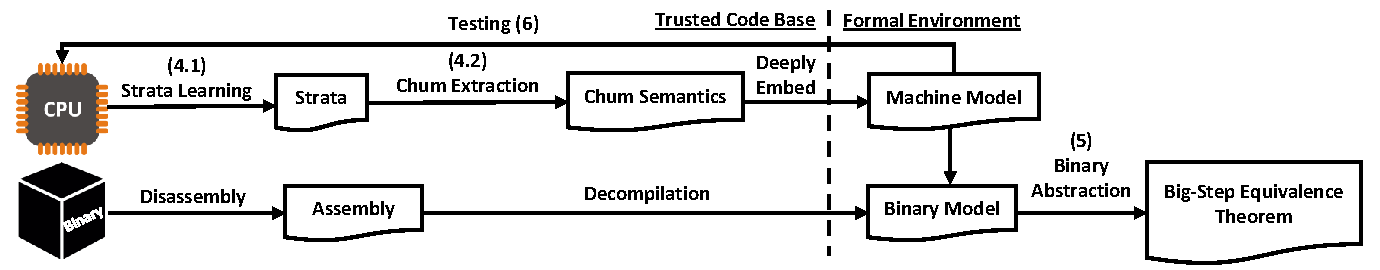
\includegraphics[width=\linewidth]{Overview_wide.pdf}
\caption{Methodology to lift abstract specifications out of x86-64 binaries}
\label{fig:method_overview}
\end{figure*} 


The first step is \emph{reassembly} (see Figure~\ref{fig:method_overview}).
Various reassemblers exist, e.g., IDA Pro \cite{eagle2011ida}, Ramblr \cite{wang2017ramblr}, Capstone \cite{quynh2014capstone}, and Codesurfer \cite{balakrishnan2005codesurfer}.
Reassembly provides \emph{symbolization}.
Symbolized assembly ensures memory references are translated from concrete addresses to labels.
Effectively, this reverses the memory layout step a compiler takes when translating a source to binary.
Symbolization supports formal verification that is agnostic of memory layout.
%The disassembler is part of the TCB: a formally verified disassembler is out of the scope of this paper.
%However, it is possible to recompile the disassembled file into a binary. 
%Our methodology requires two properties: \emph{symbolization} and \emph{re-compilation}.
%Re-compilability provides an argument toward removal of the disassembler from the TCB, as it provides the capability to reproduce the initial pre-disassembled binary.
We use Ramblr, built upon Capstone.
Ramblr provides sufficient symbolization, and provides recompilable assembly. %, and given its available source code was modifiable to support addition of annotations in comment fields to support formal verification efforts.

We perform a \emph{deep} embedding of the reassembled binary into Isabelle/HOL data structures.
A deep embedding is a simple syntactic translation requiring only a parser.
This reduces the TCB, as it prevents semantical errors in the translation.
%A deep embedding is a simple syntactic translation requiring only a parser.
%This reduces the TCB, as it prevents semantical errors in the translation. %This is ideal as it provides minimal opportunity for modification to the semantics intent of the assembly code, reducing the TCB.
%In the absence of a ready off-the-shelf grammar we developed one to support the assembly parser.
The result is a \emph{binary model}: a populated data structure in Isabelle/HOL, which contains the text-, data- and bss-sections of the binary.
Section~\ref{sec:binary_model_overview} provides more details.

%The next step is to provide semantics for the binary model.
%In order to investigate dynamical behavior of binaries over state transition, a formal model of computation is required.
%Our formal model of computation is split into a Machine model and a Binary model.
%This requires a \emph{machine model} for the x86-64 architecture.
%A machine model provides a step function that transforms the state given a single instruction.
%The x86-64 instruction set architecture (ISA) -- as of the Kaby Lake architecture -- provides a significant %amount of instruction mnemonics (1008) and variants (3720).
%Their specifications are codified within Intel reference manuals, in informal language.
%Translating these manually to Isabelle/HOL is error-prone and requires human interpretation of the reference %manuals.

To build a machine model, we leverage Strata \cite{heule2016}. 
Strata provides highly trustworthy semantics of x86-64 instructions that have been obtained by machine learning.
%The machine learned semantics are proven equivalent to hand-written semantics, using SMT solvers.
Strata demonstrates trustworthy semantics for 692 instructions, which through generalization arguments expands to 1625 IVs.
An additional 119 instructions with 8-bit immediate operands are supported by providing 256 formulas per instruction (one formula per immediate value).
%An additional 119 instructions with 8-bit immediate operands were learned piece wise, through the production of 256 separate formulas. 

We \emph{extract} generalized semantics out of Strata.
The semantics in Strata are stored either as assembly code fragments that derive off a base set of instructions, or as functions within \CC.
Strata has an application that can translate the aforementioned into bit-vector formulas for a specific instruction.
However, there was no support for memory operands and the output was specific to the supplied set of operands.
We developed a tool in the Strata \CC~ namespace that implements the generalization arguments for memory and immediate arguments, and outputs formulas for 1625 IVs in a form generic with respect to operands (see Section~\ref{sec:strata->chum}).
For instructions unsupported by Strata (e.g., jumps), we define hand-written semantics.

We developed a formal language called \emph{Chum} that can be used to express x86-64 instruction semantics.
Chum serves as an intermediary between Strata and Isabelle/HOL.
It combines standard bit-vector formulas (such as in QF\_BV in SMT-LIB~\cite{barrett2010smt}) with our machine model.
It thus contains operators to update the machine state, such as memory read/writes, and register- and flag assignments.
We extract Chum from Strata.
The result -- a file containing instruction semantics written in Chum -- is then deeply embedded into Isabelle/HOL.
%That produces a populated Chum data structure.
%That data structure is given semantics.
Essentially, this methodology reduces the problem of giving semantics to the full x86-64 instruction set to giving semantics to a small bit-vector language.
%Section~\ref{sec:machine_model} presents this approach.
To minimize the TCB, a testing framework is set up to test the formal instruction semantics on an actual x86-64 machine (see Section~\ref{sec:testing}).

The result of these steps is a trustworthy syntactical representation of a binary in Isabelle/HOL, with trustworthy semantics for each individual instruction.
The next step is to derive big-step semantics of blocks within the binary (see Section~\ref{sec:block_semantics}).
We restrict the semantics of Chum to the executable subset of the logic of Isabelle/HOL wherever possible.
Moreover, we provide a library of rewrite rules proven correct within Isabelle/HOL.
This allows formal symbolic execution, which automatically rewrites the per-instruction small-step semantics to big-step block semantics.


%Found within the TCB is the kernel of the theorem prover, in our case Isabelle/HOL, and the parser to deeply embed our binary. As mentioned, we minimize the trust of the parsers through the use of deep embeddings. Through the use of a re-compilable disassembler we remove the disassembler from the TCB. Lastly, through re-validating the original Strata test cases as test lemmas within Isabelle /HOL we remove all the intermediary steps between Strata to Isabelle from the TCB.


\section{Overview of Formal Model}\label{sec:overview}

\subsection{Machine Model}\label{sec:machine_model_overview}

%The model consists of two parts: a \emph{machine model} and a \emph{binary model}.
The machine model $\mathcal{M}$ consists of a state automaton with instructions as labels.
The set of states $S$ is a defined using a record.
Let $R_n$ denote the set of $n$-bit registers and $F$ denote the set of flags.
We use the Isabelle datatype $'\alpha~\var{word}$~\cite{dawson2009isabelle} to define bit-vectors of length~$'\alpha$.
\[
\begin{array}{l}
	S \equiv~
    <\!\var{regs} :: R_n \mapsto \bv{n},  \var{mem} :: \bv{64} \mapsto \bv{8}, \\
    \mbox{\hspace{5ex}}\var{flags} :: F \mapsto \mathbb{B}\!>
	\mbox{\hspace{3ex}with~} n \in \{64,256\}
\end{array}
\]

The state stores the contents of the registers, provides a 64-bit address space of bytes, and stores the flags.
To access a part of the state $\sigma$, read and write functions $r$ and $w$ are defined. For example, $r(\mathtt{rip}, \sigma)$ reads the instruction pointer register and $w(a,255,\sigma)$ writes at address $a$ the byte $255$ into memory.
Note that there are no registers smaller than 64 bits, nor are there 128-bit registers.
For example, the 32-bit register $\mathtt{eax}$ is a part of the 64-bit $\mathtt{rax}$ register.
The semantics of instructions concerning $\mathtt{eax}$ are thus expressed in terms of operations on the 64-bit $\mathtt{rax}$ register.
For example, writing the 32-bit register $\mathtt{eax}$ will additionally zero out the remaining 32 bits of $\mathtt{rax}$, whereas writing to the 16-bit $\mathtt{ax}$ will zero out the upper 32 bits but leave the remaining 16 bits of the lower part untouched.
Similar semantics exist for 128-bit registers, which are actually part of the 256-bit ones.
Finally, we introduce functions $r_\var{mem}$ and $w_\var{mem}$ to read and write blocks of bytes to the memory at once.
For example, $w_\var{mem}(v, a, s, \sigma)$ writes -- in little-endian fashion -- value $v$ into the memory at address $a$, split into a list of $s$ bytes.
Depending on the size, the value is possibly truncated or zero-extended.

The machine model is a step function over these states labeled with assembly instructions.
Let $I$ denote the set of instructions:
\[
	\mathcal{M} :: I \times S \mapsto S
\]
An instruction is determined by its \emph{instruction variant} (IV) and its \emph{operands}.
For example:\\
\begin{tabular}{ll}\hline
Instruction:  & \texttt{add rax, rbx} \\
Variant: & \texttt{add r64, r64} \\
Operands: & [\texttt{rax},\texttt{rbx}] \\\hline
Instruction: & \texttt{cmp	dword ptr [rbp - 0x14], 0x7F} \\
Variant:   	& \texttt{cmp m32, imm32} \\
Operands: &  [\texttt{dword ptr [rbp - 0x14]},\texttt{0x7F}] \\\hline
\end{tabular}\\
The type $V$ is used to denote the set of IVs and the operands.

\subsection{Chum: Instruction Semantics}\label{sec:machine_model}

%In this section we define the syntax of chum, provide an overview of the data structures associated with Chum embedded in Isabelle/HOL, and conclude with Machine Model definitions for $\var{getChum}$ and $\var{close}$. 
%We then follow with a sub-section outlining how we leverage Strata to acquire verified semantics, lift the results into an Isabelle/HOL datatype $\mathtt{semantics}$, evaluate . We then discuss the evaluation of conclude with defining $\var{getChum}$.
%Our small step semantics are codified in plain-text language we define called "Chum". 
%Chum is designed to be a portable reference langage for x86-64 semantics. 
%At a broad level, chum encodes sets of semantics parameterized over operands describing the behavior of a particular IV. 
%Each semantics is defined as a set of independent assignments to registers, flags, and memory portions required to execute a particular instruction. 
Central to the machine model is a function $\var{getChum} :: V \mapsto \var{Chum}$.
The semantics of an instruction are fully determined by its IV.
The semantics are expressed by a datatype $\var{Chum}$ assigning bit-vector formulas (bvf) to registers and flags (see Figure~\ref{fig:grammar}).
The sequence of bvfs of a certain IV is executed \emph{independently}, i.e., all assignments occur simultaneously on the state.

\begin{figure}[thb]
\[
\hspace{-1ex}
\begin{array}{lcl}
%	\mathtt{semantics} 	&\rightarrow& \multicolumn{2}{l}{(\mathtt{instruction\_variant},~\mathtt{chum})\mid \mathtt{semantics} ; \mathtt{semantics}}\\
	\mathtt{chum} \hspace{-1.5ex}&\rightarrow&\hspace{-1.5ex} \mathtt{assignee} \coloneqq \mathtt{bvf}\mid \mathtt{semantic} ; \mathtt{semantic}\\
	\mathtt{assignee} \hspace{-1.5ex}&\rightarrow&\hspace{-1.5ex} \mathtt{reg} \mid \mathtt{mem} \mid \mathtt{flg} \mid \mathtt{var} \\	
	\mathtt{mem} \hspace{-1.5ex}&\rightarrow&\hspace{-1.5ex} (\mathtt{loc}, \mathbb{N}) \\
	\mathtt{loc} \hspace{-1.5ex}&\rightarrow&\hspace{-1.5ex} \mathtt{loc}~\Box_a~\mathtt{loc} \mid 64~\var{word} \mid [\mathtt{reg}] \mid \mathtt{label} \\
	\mathtt{bvf} \hspace{-1.5ex}&\rightarrow&\hspace{-1.5ex} \mathtt{bvf}~\Box_b~\mathtt{bvf} \mid \Box_u(\mathtt{bvf}) \mid \mathtt{bvf} \testbit \mathbb{N} \mid \mathtt{val}\\
	 &&\hspace{-1.5ex}\mid \langle \mathbb{N}, \mathbb{N}\rangle \mathtt{bvf}	 \mid \bitmoded{\mathbb{N}}{\mathtt{bvf}} \mid \mbox{if~} \mathtt{Bbvf} \mbox{~then~} \mathtt{bvf} \mbox{~else~} \mathtt{bvf}  \\
	\mathtt{Bbvf} \hspace{-1.5ex}&\rightarrow&\hspace{-1.5ex} \mathtt{bvf}~\Box_B~\mathtt{bvf} \\
	\mathtt{val} \hspace{-1.5ex}&\rightarrow&\hspace{-1.5ex} \mathtt{var} \mid \mathtt{closed} \\
    \mathtt{var} \hspace{-1.5ex}&\rightarrow&\hspace{-1.5ex} \var{OP1} \mid \var{OP2} \mid \var{OP3} \\
     \mathtt{closed}\hspace{-1.5ex}&\rightarrow&\hspace{-1.5ex} r(\mathtt{reg}, \sigma) \mid r_\var{mem}(\mathtt{mem},\sigma)	\mid \mathtt{imm}\\
\multicolumn{3}{l}{\mbox{\hspace{3ex}where}}\\
\multicolumn{3}{l}{\Box_a \hspace{-0.5ex}\in \hspace{-0.5ex}\{+,-,* \}, \Box_b \in \{+,-, \wedge, \vee, _\smile,<\!<, +^f, -^f,...\}}\\
\multicolumn{3}{l}{\Box_u \hspace{-0.5ex}\in \hspace{-0.5ex}\{\ucast, \sextend, \neg, \parity, |\_|^f \}, \Box_B \in \{ =, \neq, \geq, \leq,... \}}
\end{array}
\]
\caption{Chum Grammar}
\label{fig:grammar}
\end{figure}


\begin{example}
The semantics of the instruction \texttt{add rax, rbx} are the same, regardless of which 64-bit registers are used.
Function $\var{getChum}$ returns:
\\[1em]$
	 \var{getChum}(\mathtt{add~r64,~r64}) = (\var{OP1} \coloneqq \var{OP1} + \var{OP2} ; \var{ZF} \coloneqq \ldots ; \ldots)
$\\[1em]
The instruction writes the sum (a function over bit-vectors) of the operands to its first operand, and sets various flags.
\end{example}

At the top-level, Chum expresses semantics by assigning bvf's to parts of the state: registers, memory, or flags.
The assignee can also be left open.
A memory location is expressed by an address and a size.
The x86-64 instruction set allows address computation within an instruction: addresses can be computed using immediate values, values stored in registers, or labels.
A bvf consists of standard bit-vector operations such as logical and arithmetic operators, concatenation ($_\smile$), shifting, etc.
The notation $\langle h,l \rangle$ denotes bit slicing: it takes the part of the bit-vector starting at bit $l$ (from right to left) and ending at bit $h$.
The notation $\bitmoded{n}{\var{bvf}}$ is used to denote that a bit-vector formula $\mathtt{bvf}$ is in $n$-bit mode.
The parity function is used to express whether the number of set bits in the given bvf is odd.
Floating point operations are indicated by $^f$, e.g., $|a|^f$ denotes the floating point absolute function.
The unary operator $\testbit$ expresses the $n$th bit of the given bvf, starting at the right.
%This notation is used for constants, which will be zero-extended when necessary, and for \emph{casting}.
%This context-free grammar serves as the basis for storing the Chum at-rest. 
%It also serves as the basis for tools to parse and serialize Chum out of Strata and in to Isabelle/HOL data structures.

This grammar is the base for several artifacts: first, Chum extraction code writes a plain-text file containing a list of pairs of IVs and Chum semantics, based on this grammar.
Second, the grammar is defined as a Chum datatype in ML.
Third, the grammar is mechanized as a grammar file for the MLTON compiler.
MLTON then generates a parser that reads in the plain-text file, and produces a populated Chum datastructure in ML.
Effectively, this deeply embeds the semantics extracted from Strata into ML.
Fourth, the grammar is defined as a Chum datatype in Isabelle/HOL.
The Chum datastructure in ML is then deeply embedded into the Isabelle/HOL datastructure.
The list of pairs is embedded as a map, producing the function $\var{getChum}$.

\subsubsection*{Floating Point Operations}\label{subssubec:fp}
To the best of our knowledge, there is no word-level floating point library in Isabelle/HOL.
Operations are needed such as: $+^f~::~64~\mathtt{word} \times 64~\mathtt{word} \mapsto 64~\mathtt{word}$.
Defining a library for these functions is outside of the scope of this paper.
Therefore, these operations are introduced as \emph{constrained functions}.
In Isabelle, a \emph{locale} is added~\cite{ballarin2003locales}, which is a method for providing a context where some functions are introduced without a function body.
One can then formulate constraints over these functions.
To ensure that these constraints are not internally inconsistent, a witness for these functions is provided.

The floating point locale defines functions $+^f, -^f, *^f, \div^f$ over 64-bit words, representing double precision floating point operations.
Besides these, the constants $0^+, 0^-, \infty^+, \infty^-$ and functions $\sign$, $\isNaN$, and $|\_|^f$ are introduced regularly, i.e., with a concrete meaning.
Respectively, they return the sign bit (bit 63), check whether the exponent consists solely of 1's and the mantissa is non-zero, and compute the absolute value by setting the sign bit to 0.
The constraints are based on the IEEE 754-2008 standard~\cite{4610935}.
Examples are:
\begin{eqnarray*}
x +^f 0^+ \hspace{-1ex}&\equiv& \hspace{-1ex} x \\
x *^f 0^+ \hspace{-1ex}&\equiv& \hspace{-1ex}\mbox{if~} \sign(x) \mbox{~then~} 0^+ \mbox{~else~} 0^-\\
x \notin \{0^+,0^-\} \Longrightarrow x \div^f 0^+ \hspace{-1ex}&\equiv&\hspace{-1ex} \mbox{if~} \sign(x) \mbox{~then~} \infty^- \mbox{~else~} \infty^+\\
\{x, y\} \subseteq \{0^+,0^-\} \hspace{-1ex}&\Longrightarrow&\hspace{-1ex} \isNaN(x \div^f y)
\end{eqnarray*}
The effect of using this locale instead of concretely defined functions, is that they are not executable.
For the constrained functions, we can symbolically execute and simplify floating point formulas only based on the rules introduced by the locale.
We will show in Section~\ref{sec:block_semantics} that we can derive floating point formulas out of a binary.
However, floating point constants are simply bit-vectors represented by hexadecimal numbers.

\subsection{Decompilation-into-logic}\label{sec:binary_model_overview}

The binary model $\mathcal{B}$ consists of the instructions to be executed, an initial state, and a termination condition.
Let $A$ denote the address space, i.e, $A = \bv{64}$.
\[
	\mathcal{B} \equiv~<~\var{fetch} :: A \mapsto I, \var{\sigma_0} :: S, \var{is\_final} :: A \mapsto \mathbb{B}>
\]
Function $\var{fetch}$ provides the current instruction to be executed, based on the current $\mathtt{rip}$.
The initial state is obtained by loading all data- and bss sections of the binary into memory.
The termination condition decides when the binary is finished based on an address.

In order to build the binary model in Isabelle/HOL, a datatype is built that can store a deep embedding of the binary.
The datatype consists of datatypes for instructions, registers, flags, address computations, labels, and immediates.
Using the MLTON parser generator\footnote{See: \url{mlton.org}}, a parser for x86-64 \texttt{.s} assembly files is built.
Via ML, this parser then generates a populated data structure within Isabelle/HOL.
We have added a command to Isabelle/HOL called \texttt{x86\_64\_parser} which takes as input the name of an assembly file and loads it into the theorem prover.

We source the \texttt{.s} assembly files from an x86\_64 binary using the Ramblr disassembler.
Ramblr is modified to automatically add annotations in comment fields, which are deeply embedded along with the assembly.
The instruction size is added in bytes.
This is used to increment \texttt{rip} and to compute relative offsets for branching instructions.
The opcode is added as well.
An opcode is what tells the hardware exactly what operation to perform.
Within the Intel ISA there are cases were the hardware has multiple opcodes which support the same instruction, often for optimization purposes.
For example instruction \texttt{ror ax, 1} (Rotate Right) can be supported by two different opcodes (0xD1 and 0xC1) as there is an optimized version of the ror instruction for shifts of value 1.
Instruction \texttt{ror ax, 2} has support by only one opcode (0xC1).
%SPACE
%In our modified Ramblr this latter example would be disassembled as:
%\[
%\texttt{ror ax, 2\hspace{6ex} \#  Size:4, Opcode: 0xC1}\\
%\]
While it is generally assumed that multiple opcodes supporting the same instruction behave identically, this additional information is necessary for a full deep embedding of the binary within Isabelle/HOL.

What it means to run a binary on top of a machine can now be defined:
\[
\begin{array}{lcl}
\var{start} & = & \var{run}(\mathcal{B}.\sigma_0)\\
\var{run}(\sigma) & = & \mbox{let~} \var{rip} = r(\mathtt{rip}, \sigma) \mbox{~in} \\
	&& \mbox{\hspace{2ex}if~} \mathcal{B}.\var{is\_final}(\var{rip}) \mbox{~then~} \sigma\\
	&& \mbox{\hspace{2ex}else~} \var{run}(\mathcal{M}(\mathcal{B}.\var{fetch}(\var{rip}),\sigma))
\end{array}
\]

\section{Extraction of Chum from Strata}\label{sec:strata->chum}

\subsection{Strata and Stoke Introduction}

We leverage the semantics machine learned by Strata \cite{heule2016} from x86-64 hardware.
%It uses a stochastic search methodology.
The search space in which the instructions are learned is a subset of the assembly language (strataAL) consisting of sequential permutations of 51 assumed correct hard-coded register-only instructions and 11 pseudo-instructions (i.e., the \emph{base set}).
%These base/pseudo instructions, hereafter referred to as the \emph{base set}, cover integer arithmetic, bitwise operations, data movement, floating point operations, splitting and combining of registers, and setting and clearing of status flags. 
%The base set covers fundamental operations serving as building blocks for the more complex instructions that are ultimately learned as assembly code fragments. 
%Within the base set are uninterpreted functions to model floating points. 
%This allows to learn semantics of SIMD floating point instructions, even though these semantics are not executable.
%Uninterpreted functions while imprecise, are sufficient to learn relationships between vectored versions of base instructions containing these uninterpreted functions. 
Strata uses a compiler optimization tool called Stoke~\cite{schkufza2013stochastic} to learn IVs as strataAL fragments. 
Stoke requires as input a set of test cases (input/output pairs).
Initially it uses random test cases, with some additional special test cases to cover common corner cases or register values. 
Strata uses Stoke to learn multiple strataAL fragments for a given instruction.
Based on the stochastic nature of the search, each of these learned strataAL fragments can produce different results. Strata then uses the Z3 SMT solver~\cite{de2008z3} to prove equivalence between these learned strataAL fragments. 
If the SMT solver proves non-equivalence, a counterexample is then fed back into the test cases, and the process repeats.
Ultimately the test cases we use to validate our machine model are concolic versions of these test cases Strata learned as part of this counterexample guided refinement, along with the initial random test cases, and heuristically interesting cases. 
%As instructions are utlearned as strataAL fragments, they are fed back into the base set, expanding the expressability of strataAL on which to learn subsequent instructions.
%Useful after generalization argument discussion
%They were able to learn support for approximately 60\% of the remaining 2,918 IVs within the Haswell ISA.

In total, Strata learns 692 instructions (one per each register-only IV).
Specifically excluded from their learning were MMX, cryptography, x87, \texttt{loop}, string instructions (including the \texttt{rep} prefix), and any post-Haswell ISA instructions. 
 Included are SSE (2 -- 4.1), AVX, AVX2, FMA3, BM1, BM2, as well as legacy x86 instruction sets.  

Strata's x86-64 semantics are stored in two different forms. The learned semantics are stored as non-looping strataAL fragments. 
The initial base set and pseudo instructions are stored as manually written semantics composed as \CC~ code.
Stoke has an application called \texttt{stoke\_debug\_circuit} that can produce a bit-vector formulas (bvf) for a learned instruction given its associated strataAL fragment.
All formulas produced operate on either whole 64-bit or 256-bit registers. 
For example, the bvf for the 32-bit \texttt{add eax, ebx} will provide a formula that writes to the 64-bit \texttt{rax} register. 

It is not possible to directly leverage either the learned semantics or the \texttt{stoke\_debug\_circuit} application, to extract all the semantics from Strata.
This is because:
\begin{enumerate}
\item The semantics are not in a form that can be directly parsed and leveraged into logic. 
As mentioned, they are stored as non-looping register-only assembly code fragments (strataAL), or \CC~ code. 
%\item The strataAL form is not generalized over arbitrary registers and operand types.
\item The \texttt{stoke\_debug\_circuit} application lacks support for production of bit-vector formulas that write to memory. For example, it is unable to produce a formula for the following instruction: 
\texttt{sal m64, imm8}.
\item The \texttt{stoke\_debug\_circuit} application produces formulas for \emph{instructions}. For tractability, we require formulas generalized to IVs. 
When one considers instructions with immediate values, this generalization is more complex than a simple symbolic match-and-replace. 
Consider the IV \texttt{sal r64, imm8}.
Stimulating the application, for this IV, with operands $\mathtt{rbx}$ and $\mathtt{1}$, produces the following bvf: 
\[
\begin{array}{lcl}
\mathtt{rbx} & \coloneqq & \langle 63,0\rangle(\bitmoded{1}{0} {_\smile} \mathtt{rbx} <\!< \bitmoded{57}{0} {_\smile} \bitmoded{8}{1})
%\mathtt{rcx}:& &(0x0\_1 \hspace{1.5ex} \mbox{o} \hspace{1.5ex} \mathtt{rcx} \hspace{1.5ex} << \hspace{1.5ex} 0x0\_57 \hspace{1.5ex} \mbox{o} \hspace{1.5ex} 0x1\_8)[63:0] \\
\end{array}
\]
Trivially, \texttt{rbx} can be replaced with symbol \texttt{OP1} to represent operand 1. 
In terms of the immediate, one might assume that substituting the 8-bit value 1 with symbol \texttt{OP2} would suffice.
Consider, however the same IV when stimulated with \texttt{rbx} and an immediate value of 0xFF:
\[
\begin{array}{lcl}
\mathtt{rbx} & \coloneqq & \langle 63,0\rangle(\bitmoded{1}{0} {_\smile} \mathtt{rbx} <\!< \bitmoded{57}{0} {_\smile} \bitmoded{8}{0x3F})
%\mathtt{rcx}: \hspace{1.5ex} (0x0\_1 \hspace{1.5ex} \mbox{o} \hspace{1.5ex} \mathtt{rcx} \hspace{1.5ex} << \hspace{1.5ex} 0x0\_57 \hspace{1.5ex} \mbox{o} \hspace{1.5ex} 0x3F\_8)[63:0] \\
\end{array}
\]
This case demonstrates that generalization cannot be achieved by a simple match-and-replace, as value 0xFF is not found in the formula produced.
This example will be revisited in the next section, as we discuss our approach for extracting semantics out of Strata.
\end{enumerate}

\subsection{Chum Extraction}\label{subsec:chumextraction}

We extract bit-vector formulas from Strata, per IV, into a serialized version of Chum. % for a deep embedding into Isabelle/HOL. 
For register-only IVs, generating the bvf is accomplished by stimulating \texttt{stoke\_debug\_circuit} with an instruction that consists of the IV instantiated with \emph{safe registers}.
A match-and-replace is then done from the safe registers to open variables.

In choosing specific operands for the instruction to be learned, registers were chosen such that they would \emph{generalizable}. 
For example, \texttt{rbx} and \texttt{rcx} were the chosen operands utilized when learning binary register-only 64-bit IVs. 
These are safe registers, as these registers are never directly written to unless specified as operands. 
As a counterexample, \texttt{rax} is an unsafe register as \texttt{cmpxchg} directly writes to it regardless of whether \texttt{rax} is provided as an operand.

Consider the following example, which generates the bvf for \texttt{add r64, r64}.
Application \texttt{stoke\_debug\_circuit} is stimulated with \texttt{add rbx, rcx}, which produces the following bvf:
\[
\begin{array}{llcl}
\mathtt{add\hspace{0.5ex} rbx, rcx}: 
& \mathtt{rbx} &\coloneqq& \langle 63, 0 \rangle(\bitmoded{1}{0} {_\smile} \mathtt{rbx} + \bitmoded{1}{0} {_\smile} \mathtt{rcx})
%\mathtt{rbx}:& &(0x0\_1 ~\mbox{o}~ \mathtt{rbx} ~+~ 0x0\_1 ~\mbox{o}~ \mathtt{rcx})[63:0]\\
\end{array}
\]
This is match-and-replaced to:
\[
\begin{array}{llcl}
\mathtt{add\hspace{0.5ex} r64, r64}: 
& \mathtt{OP1} &\coloneqq&\langle 63, 0 \rangle(\bitmoded{1}{0} {_\smile} \mathtt{OP1} + \bitmoded{1}{0} {_\smile} \mathtt{OP2})
%\mathtt{OP1}:& &(0x0\_1 ~\mbox{o}~ \mathtt{OP2} ~+~0x0\_1 ~\mbox{o}~  \mathtt{OP1})[63:0]\\
\end{array}
\]
For non-register-only IVs, the extraction process is more involved. 
Each IV, $\var{iv}$, is mapped to a register-only IV that \emph{supports} it, $\var{iv'}$. 
An IV, $\var{iv'}$, supports $\var{iv}$ if $\var{iv'}$ has the same mnemonic, number of operands, and each operand meets specific criteria for generalization.
An operand in $\var{iv}$ does not require generalization support if it is already a register.
For a non-register operand, the criteria are based on its type and bit-length, as well as those of the corresponding register operand of $\var{iv'}$.
The semantics for instruction~$\var{iv}$ are obtained by stimulating \texttt{stoke\_debug\_circuit} with $\var{iv'}$ with safe registers, which are then match-and-replaced to open variables.
Lastly, any operand size mismatches between the supporting and supported operands are resolved. 
We will now discuss the criteria for operand generalization and any required size mismatch resolution.

\subsubsection*{Generalization to immediate operands.} 
The register operand providing support for the immediate must be of equal or greater size. Consider the example from the previous section \texttt{sal r64, imm8}. 
This variant finds support from the variant \texttt{sal r64, r8}.
Application \texttt{stoke\_debug\_circuit} is stimulated with \texttt{sal rbx, cl}, which produces the following bvf:
\[
\begin{array}{llcl}
\mathtt{sal\hspace{0.5ex} rbx, cl}: \\
 \hspace{3ex}\mathtt{rbx} \coloneqq  \langle 63,0\rangle(\bitmoded{1}{0} {_\smile} \mathtt{rbx} <\!< \bitmoded{57}{0} {_\smile} (\langle 7,0\rangle\mathtt{rcx} ~\wedge~ \bitmoded{8}{0x3F}))
\end{array}
\]
Doing the match-and-replace yields:
\[
\begin{array}{llcl}
\mathtt{sal\hspace{0.5ex}} \mathtt{r64, imm8}: \\
 \hspace{3ex} \mathtt{OP1}  \coloneqq  \langle 63,0\rangle(\bitmoded{1}{0} {_\smile} \mathtt{OP1} <\!< \bitmoded{57}{0} {_\smile} (\langle 7,0\rangle\mathtt{OP2} ~\wedge~ \bitmoded{8}{0x3F}))
%\mathtt{OP1}:& &(0x0\_1 ~\mbox{o}~ \mathtt{OP2} ~+~0x0\_1 ~\mbox{o}~  \mathtt{OP1})[63:0]\\
\end{array}
\]
Operator $\wedge$ denotes standard bit-vector conjunction. 
As there was no size mismatch between~\texttt{cl} and~\texttt{imm8} nothing further is required.
In case of a size mismatch, a sign extension is introduced into the bvf after it is returned from \texttt{stoke\_debug\_circuit}.
Consider $\mathtt{add~r32, imm8}$.
It is supported by $\mathtt{add~r32, r32}$.
Semantics are extracted by generalizing to open variables, and introducing sign-extension:
\[
\begin{array}{llcl}
\mathtt{add\hspace{0.5ex} ebx, ecx}:  \\
  \hspace{1ex}\mathtt{ebx} \coloneqq \bitmoded{32}{0} {_\smile} \langle 31,0\rangle(\bitmoded{1}{0} {_\smile} \langle 31,0\rangle\mathtt{ecx} + \bitmoded{1}{0} {_\smile} \langle 31,0\rangle\mathtt{ebx}) \\
 
\mathtt{add\hspace{0.5ex}} \mathtt{r32,imm8}: \\
   \hspace{1ex} \mathtt{OP1} \hspace{-0.5ex}\coloneqq \bitmoded{32}{0} {_\smile} \langle 31,0\rangle(\bitmoded{1}{0} {_\smile} \langle 31,0\rangle\bitmoded{32}{\sextend(\mathtt{OP2})} + \bitmoded{1}{0} {_\smile} \langle 31,0\rangle\mathtt{OP1})\\ 
 %\hspace{3ex} \mathtt{OP1} = 0x0\_32 \hspace{0.5ex} \mbox{o} \hspace{0.5ex} (0x0\_1\hspace{0.5ex} \mbox{o} \hspace{0.5ex} \sextend(\mathtt{OP2},32)[31:0]\hspace{0.5ex} +\hspace{0.5ex} 0x0\_1\hspace{0.5ex} \mbox{o} \hspace{0.5ex} \mathtt{OP1}[31:0])[31:0]
\end{array}
\]
\subsubsection*{Generalization to memory operands.}
Similar to the immediate case, the register operand providing support for the memory operand must be of equal or greater size. 
As memory operands can be written to, this generalization has another case to consider in resolving operand size mismatches.
If the supporting operand is being written to, a slicing operator is introduced, truncating the bit-vector to the appropriate size. 
Consider IV \texttt{movapd m128,xmm}.
This is supported by \texttt{movapd xmm,xmm}.
Application \texttt{stoke\_debug\_circuit} is stimulated with safe xmm-registers \texttt{xmm1} and \texttt{xmm2}. 
\[
\begin{array}{llcl}
\mathtt{movapd\hspace{0.5ex} xmm1, xmm2}:
	 \mathtt{ymm1} \coloneqq \langle 255,128\rangle \mathtt{ymm1} {_\smile} \langle 127,0\rangle\mathtt{ymm2}\\
% \hspace{3ex} \mathtt{OP1} = \mathtt{OP1}[255:128] ~\mbox{o} ~ \mathtt{OP2}[127:0]\\ 
\mathtt{movapd\hspace{0.5ex} m128,xmm}: \\
	 \hspace{1ex}\mathtt{OP1} \coloneqq \langle 127,0\rangle(\langle 255,128\rangle \mathtt{OP1} {_\smile} \langle 127,0\rangle\mathtt{OP2})
% \hspace{3ex} \mathtt{OP1} = (\mathtt{OP1}[255:128] ~ \mbox{o} ~ \mathtt{OP2}[127:0])[127:0]\\ 
\end{array}
\]
%In this example, even though the operands are the same size, due to the fact that registers are always operated on by their parent 64-bit or 256-bit register, a slicing occurs. 
In case the supporting register operand is larger than the supported memory operand, the upper parts of the register are truncated.
This means that no further steps are required.
Consider the following example for \texttt{addsd xmm,m64} which is supported by \texttt{addsd xmm,xmm}:
\[
\begin{array}{llcl}
\mathtt{addsd\hspace{0.5ex} } \mathtt{xmm1, xmm2}: \hspace{1.0ex} \mathtt{ymm1} \coloneqq \langle 255,128\rangle \mathtt{ymm1} {_\smile}\\
	    \hspace{6ex} \langle 127,64\rangle \mathtt{ymm1} {_\smile} (\langle 63,0\rangle\mathtt{ymm1} +^f \langle 63,0\rangle \mathtt{ymm2}) &\\
 %\hspace{3ex} \mathtt{OP1} = (\mathtt{OP1}[255:128] ~ \mbox{o} ~\mathtt{OP1}[127:64] ~ \mbox{o} ~ \mbox{add\_double}(\mathtt{OP1}[63:0], \mathtt{OP2}[63:0]))\\ 
\mathtt{addsd\hspace{0.5ex}} \mathtt{xmm,m64}: \hspace{1.0ex}\mathtt{OP1} \coloneqq\\
	    \hspace{2.0ex} \langle 255,128\rangle \mathtt{OP1} {_\smile} \langle 127,64\rangle \mathtt{OP1} {_\smile} (\langle 63,0\rangle\mathtt{OP1} +^f \langle 63,0\rangle \mathtt{OP2}) &
 %\hspace{3ex} \mathtt{OP1} = (\mathtt{OP1}[255:128] ~ \mbox{o} ~\mathtt{OP1}[127:64] ~ \mbox{o} ~ \mbox{add\_double}(\mathtt{OP1}[63:0], \mathtt{OP2}[63:0]))\\ 
\end{array}
\]
For some instructions, we do not use learned semantics.
Some instructions have no Strata support.
For these, we supply manually written semantics.
For another 119 IVs (with 8-bit immediate operands), there is no register-only equivalent.
For these IVs, Strata learns 256 distinct formulas per variant.
Our methodology does not support these ``brute-forced'' formulas. 
We drafted manual semantics to support branching instructions such as jump and call, as well as stack operating instructions such as push and pop. 
The learned semantics of the parity flag are impractical for theorem proving, since they produce very large bit-vector formulas. We therefore express the semantics of the parity flag manually.

Figure~\ref{fig:learned_semantics_sub} shows the semantics of the \texttt{sub} IV after extraction from Strata and embedding within Isabelle/HOL, for a 32-bit register $\var{r32} = \langle 31,0\rangle r(\var{r64}, \sigma)$ and a 32-bit memory location $\var{m32} = r_\var{mem}(\var{a},4,\sigma)$ .
The instruction causes 6 state changes: the 64-bit register $\var{r64}$ corresponding to register $\var{r32}$ is completely overwritten with a bit-vector consisting of 1.) zeroes for the upper 32 bits, and 2.) for the lower 32 bits the lower 32 bits of the result of two's complement subtraction in 33-bit mode.
The input values come from reading register $\var{r64}$ and taking the lower 32 bits and from reading 4 bytes of memory from address~$\var{a}$.
The zero flag is obtained by checking whether the result is zero, and the carry- and sign flags check respectively bits 32 and 31.
An overflow occurs when the most significant bits (msb) initially were different, whereas the msb's of the result and the initial value at $\var{a}$ are equal.
Note that we do not show the parity flag update.

\begin{figure}[htb]
\begin{tabular}{lcl}
$\var{r64}$ & $\coloneqq$ & $\bitmoded{32}{0} {_\smile} \langle 31,0\rangle(\bitmoded{1}{0} {_\smile} \neg \var{op2} + \bitmoded{33}{1} + \bitmoded{1}{0} {_\smile} \langle 31,0\rangle(\var{op1}))$\\
$\var{ZF}$ & $\coloneqq$ & $\langle 31,0\rangle(\bitmoded{1}{0} {_\smile} \neg \var{op2} + \bitmoded{33}{1} + \bitmoded{1}{0} {_\smile} \langle 31,0\rangle(\var{op1})) == \bitmoded{32}{0}$\\
$\var{CF}$ & $\coloneqq$ & $\langle 32,32\rangle(\bitmoded{1}{0} {_\smile} \neg \var{op2} + \bitmoded{33}{1} + \bitmoded{1}{0} {_\smile} \langle 31,0\rangle(\var{op1})) == \bitmoded{32}{1}$\\
$\var{SF}$ & $\coloneqq$ & $\langle 31,31\rangle(\bitmoded{1}{0} {_\smile} \neg \var{op2} + \bitmoded{33}{1} + \bitmoded{1}{0} {_\smile} \langle 31,0\rangle(\var{op1})) == \bitmoded{32}{1}$\\
$\var{OF}$ & $\coloneqq$ & $\neg \langle 31,31\rangle(\var{op2}) == \bitmoded{1}{1} \longleftrightarrow \langle 31,31\rangle(\var{op1} == \bitmoded{1}{1})~\wedge$ \\
\multicolumn{3}{l}{ $\neg(\neg(\langle 31,31\rangle(\var{op2})) == \bitmoded{1}{1} \longleftrightarrow$}\\
\multicolumn{3}{r}{$\langle 31,31\rangle(\bitmoded{1}{0} {_\smile}\neg \var{op2} + \bitmoded{33}{1} + \bitmoded{1}{0} {_\smile}\langle 31,0\rangle(\var{op1})) == \bitmoded{1}{1})$}\\
\multicolumn{3}{l}{\hspace{3ex}where $\var{op1}$  =  $r(\var{r64}, \sigma)$,   
$\var{op2}$  =  $r_\var{mem}(\var{a},4,\sigma)$}

\end{tabular}
\caption{Learned semantics of \texttt{sub~r32~m32} deeply embedded into Isabelle/HOL.}
\label{fig:learned_semantics_sub}
\end{figure}

 % Head 1
\section{Big-Step Semantics}\label{sec:block_semantics}

The machine model provides small-step semantics, i.e., semantics per instruction.
Our objective is to find a high-level representation of the big-step semantics of blocks of assembly within the binary.
Note that our definition of blocks characterizes larger chunks of the assembly than the traditional notion of ``basic blocks'', i.e., our notion of blocks also includes if-statements.
Our aim is to prove an \emph{equivalence theorem} of the form:
\[
	f(\sigma_b) = run(\sigma_b)
\]
Here, function $f$ should be defined using high-level, i.e., C-like, constructs only.
For the main function in the binary, state $\sigma_b$ will be the initial state.
For the functions in other text sections of the binary we will quantify over any state $\sigma_b$ that has the read-only data sections of the binary loaded.
This ensures compositionality.

The approach we use is \emph{formal symbolic execution}.
The symbolic execution engine needs to tackle two challenges:
\begin{enumerate}
\item Since the semantics embedded into Isabelle/HOL are generated by a machine learning algorithm (instead of being hand-written) they generally are not in a form where they can be used for theorem proving directly.
Consider, e.g., the semantics in Figure~\ref{fig:learned_semantics_sub}.
The semantics are expressed in bit-vector operations such as concatenation, bit slicing and logical operations, instead of arithmetic operations such as subtraction and (in)equality.
\item Whenever possible, the semantics of a sequence of one or more instructions needs to be simplified to a high-level operation.
\end{enumerate}
Effectively, formal symbolic execution is implemented by adding a library of formally proven correct rewrite rules to the Isabelle simplifier.
Whenever two subgoals are introduced, an if-then-else is introduced in the logic manually. 
This allows us to consider for each case whether we actually want to introduce an if-then-else, or whether we want to add a precondition that prevents one of the cases from happening.

\subsection{Formal Symbolic Execution}

The starting point is of the form:
\\[1em]
	\mbox{\hspace{5ex}} $\var{run}(\sigma_b) = \var{?f}(\sigma_b)$
\\[1em]
Here, $\var{?f}$ is a function representing the high-level semantics of the block.
Crucially, this function does not have to be defined when running symbolic execution.
It is a \emph{schematic  variable}.
A schematic variable in a lemma basically means that the final lemma as it will be proven and admitted to the Isabelle logic has not been formulated yet.
Whenever the current goal has the form $g(\sigma_b) = \var{?f}(\sigma_b)$, the proof can be stopped and the final formulation of the proven equivalence theorem becomes $\var{run}(\sigma_b) = g(\sigma_b)$.
%For example, the equivalence theorem would be trivial when function $\var{run}$ would remain untouched.
%In that case, the final formulation of the proven lemma is $\var{run}(\sigma_b) = \var{run}(\sigma_b)$, which is useless.

Symbolic execution will rewrite and simplify the left hand side of the goal.
This will rewrite $\var{run}$ to a function $f$ representing a high-level equivalent of $\var{run}$.
\begin{example}\label{ex:push_pop}
Consider the following assembly code:
\begin{lstlisting}
  push rbp
  mov  rbp, 0
  pop  rbp
\end{lstlisting}
This code first decrements the stack pointer, writes the frame pointer \texttt{rbp} into memory at location $\mathtt{rsp} - 8$, and increments \texttt{rip}.
Second, it writes the immediate value $0$ to \texttt{rbp}.
Third, it writes the value in the memory back to register \texttt{rbp}, then increments the stack pointer, and increments $\texttt{rip}$ again.
All these actions are executed symbolically.
The equivalence theorem becomes:
\\[1em]
	\mbox{\hspace{5ex}} $\var{run}(\sigma_b) = (\mathtt{rip} \coloneqq \mathtt{rip + 9} ; \mathtt{rsp} - 8 \triangleright \mathtt{rbp})(\sigma_b)$
\\[1em]
Function $f$ is represented as two state updates: register \texttt{rip} is incremented by $9$, and the frame pointer is stored in memory (notation $a \triangleright v$ denotes writing value $v$ into the memory at address $a$).
Note that both registers \texttt{rsp} and \texttt{rbp} are unchanged, even though they have been changed during execution.
\end{example}

We have developed an Isabelle \emph{proof method} using Eisbach~\cite{matichuk2016eisbach}.
A proof method is essentially a proof script that can be used to automate certain tasks.
Our proof method is called \texttt{symbolic\_execution}.
It can be applied to a goal of the following form:
\\[1em]
  \mbox{\hspace{5ex}} $\var{run}(\sigma) = f(\sigma_b)$.
\\[1em]
If the current goal has this form, method \texttt{symbolic\_execution} does the following:
\begin{enumerate}
\item Check the termination condition on state $\sigma$. In case of termination, rewrite $\var{run}(\sigma)$ to $\sigma$ and stop the proof method.
\item Fetch the next instruction based on the current state $\sigma$.
\item Check whether Strata semantics are available for that IV. If not check whether there is a manually written one available.
\item Simplify the semantics before applying them to the current state.\label{step_small_step}
\item Apply the simplified semantics to the current state $\sigma$, producing a new state $\sigma'$.
\item Simplify state $\sigma'$ to state $\sigma''$.\label{step_simplify}
\end{enumerate}
The resulting goal will be of the form $\var{run}(\sigma'') = f(\sigma_b)$, where $\sigma''$ is the result of execution of one instruction on $\sigma$.
Whenever the goals has been split into two subgoals, we either introduce an if-then-else in function $f$, or add a precondition to exclude one of the two cases.

%\begin{example}\label{ex:push_pop_rewrite}
%Consider Example~\ref{ex:push_pop}.
%After two instructions, the current state $\sigma$ will satisfy: $r(\mathtt{rsp}, \sigma) = r(\mathtt{rsp}, \sigma_b) - 8$.
%The third instruction will then execute, among others:
%\\[1em]
%	\mbox{\hspace{5ex}} $w(\mathtt{rsp}, \sigma_b, r(\mathtt{rsp}, \sigma) + 8)$
%\\[1em]
%The rewrite rule that is applied, is from the Isabelle/HOL word library:
%\\[1em]
%	\mbox{\hspace{5ex}} $\forall a, b~::~'\alpha~\var{word} \cdot (a - b) + b = a$
%\\[1em]
%Application of this rule rewrites the goal to $w(\mathtt{rsp}, \sigma_b, r(\mathtt{rsp}, \sigma_b))$, which %can be rewritten to the identity function. 
%This is why in Example~\ref{ex:push_pop} register $\texttt{rsp}$ is untouched in the big-step semantics.
%\end{example}

%Section~\ref{subsec:small_step_rewriting} provides rewrite rules that simplify the semantics of individual IVs.
%Based on those semantics, the next step is to rewrite \emph{blocks} of assembly code, thereby lifting %semantics out of the binary.
%We first explain how to apply rewriting to a block embedded into Isabelle/HOL.
%We then provide details on new rewrite rules.
%The remainder of this section demonstrates several small examples.
%The examples have been obtained by compiling source code on an x86-64 machine with \texttt{gcc} 4.2.1.
%Unless noted otherwise, we have compiled without optimization.
%Subsequently, we discard the source code and apply the methodology to the binary as if no source code is %available.
%For some examples, we show the original source code, instead of the actual text- and data sections of the %binary.
%This is due to space limitation, and because in contrast to the assembly the source code gives an intuition %of what the lifted semantics should be.
%Both the binaries and their disassembled form can be found online.
%The examples have been chosen to show how to deal with if-then-else, pointers, floating point arithmetic, %and assembly inlined in C.
%A block is defined as a sequence of instructions that can be modeled with only if-then-else statements (no %loops).
%A list of instructions without conditional jumps or calls is a block.
%Consider the following assembly sequence:
%\begin{lstlisting}
%  jb  .label0
%  (*@{\vdots\vspace*{3pt}}@*)
%  jmp label1
%.label0:
%  (*@{\vdots\vspace*{3pt}}@*)
%.label1:
%  (*@{\vdots\vspace*{3pt}}@*)
%\end{lstlisting}
%Regardless of the conditional jump, this can be considered one block as well.
%It can be modeled with an if-then-else: if the jump condition holds then block 2 is executed, otherwise %block 1.
%A block always terminates.
%We will show how to distill a high-level description of the semantics of a block of assembly out of the %small-step semantics of each individual instruction.
%The methodology is based on symbolic execution.

\subsection{Rewrite rules}

We provide some interesting examples of rewrite rules that are applied when doing symbolic execution in Figure~\ref{fig:rewrite_blocks}.
For more details and the proofs, we refer to the sources available online.

\begin{figure}[bht]
\begin{eqnarray*}
m < n \Rightarrow \langle m, 0\rangle(\bitmoded{n}{a + b}) \hspace{-7}&\equiv&\hspace{-7} \langle m,0\rangle(\bitmoded{n}{a}) + \langle m,0\rangle(\bitmoded{n}{b}) \label{eq:take_bits_plus}\\
m < n \wedge m < l \Rightarrow \langle m,0\rangle(\bitmodeu{l}{\ucast(\bitmoded{n}{a}})) \hspace{-7}&\equiv&\hspace{-7} \langle m, 0\rangle(\bitmoded{n}{a}) \\
m < n \Rightarrow \langle m, 0 \rangle(\bitmoded{n}{\neg a}) \hspace{-7}&\equiv&\hspace{-7} \neg\langle m,0 \rangle(\bitmoded{n}{a}) \label{eq:take_bits_bitNOT} \\
\langle m,0 \rangle(\bitmoded{m+1}{a}) \hspace{-7}&\equiv&\hspace{-7} \bitmoded{m+1}{a} \label{eq:remove_take_bits}\\
\neg a + 1 + b \hspace{-7}&\equiv&\hspace{-7} b - a \label{eq:tc_sub} \\
\bitmodeu{n+1}{\ucast(\bitmoded{n}{\neg a})} \hspace{-7}&\equiv&\hspace{-7} \bitmodeu{n+1}{\neg(2^n + \ucast(\bitmoded{n}{a}))}\label{eq:ucast_bitNOT}\\
\langle n,n\rangle\bitmoded{n+1}{a} \hspace{-7}&\equiv&\hspace{-7} \bitmoded{n+1}{a \geq 2^n}\label{eq:msb_is_gt_2p}\\
m < n \Rightarrow \bitmoded{n}{\ucast(\bitmodeu{m}{a}) < \ucast(\bitmodeu{m}{b})} \hspace{-7}&\equiv&\hspace{-7} \bitmodeu{m}{a} < \bitmodeu{m}{b}\label{eq:take_bits_le}\\
%(\bitmoded{n}{a} - i \leq a - j) &\equiv& \left\{\begin{array}{ll}
%	j \leq i \wedge a \geq i & \mbox{if~} a \geq j\\
%	a - i \leq (2^{n} - 1) - j + a + 1 & \mbox{otherwise}
%	\end{array}
%	\right.\label{eq:underflow}\\
%((\bitmoded{n}{a} <\!< i) = 0) &\equiv& (i \geq n \vee (\forall j < n - i \cdot \neg(a \testbit j)))\label{eq:shift_is_0}\\
%	h' < n \wedge h < h' + l + 1 &\Longrightarrow& \langle h,l\rangle\langle h',l'\rangle\bitmoded{n}{a} %\equiv \left\{\begin{array}{ll}
%	\langle h + l', l+l'\rangle a & \mbox{if~} h < h' - l'\\
%	\langle h', l+l'\rangle a & \mbox{otherwise}
%	\end{array}
%	\right.\label{eq:take_bits_take_bits}\\
%\langle h,l\rangle(a _\smile b) &\equiv& \left\{\begin{array}{ll}
%	\langle h - m, l - m\rangle a & \mbox{if~} h \geq m \wedge l \geq m\\
%				& \mbox{if~} h \geq m \wedge l  < m\\
%	0 & \mbox{if~} h < m \wedge l \geq m\\
%	\langle h, l \rangle b & \mbox{if~} h < m \wedge l  < m
%	\end{array}
%	\right. \label{eq:take_bits_cat}\\
r_\var{mem}(a,s,w_\var{mem}(v,a,s,\sigma)) \hspace{-7}&\equiv&\hspace{-7} v \label{eq:mem1}\\
(a,s) \bowtie (a',s') \Longrightarrow&&\nonumber\\
r_\var{mem}(a,s,w_\var{mem}(v,a',s',\sigma)) \hspace{-7}&\equiv&\hspace{-7} r_\var{mem}(a,s,\sigma) \label{eq:mem2}\\
(\bitmoded{n}{a} \wedge 0x7FFF\ldots) \hspace{-7}&\equiv&\hspace{-7} |a|^f  \label{eq:float_abs}\\
(|\langle 63,32\rangle \bitmoded{64}{a} \rangle|^f = \langle 31,0\rangle a = 0) \hspace{-7}&\equiv&\hspace{-7} a \in \{0^-, 0^+\}\label{eq:float_0}
\end{eqnarray*}
\caption{Examples of rewrite rules}
\label{fig:rewrite_blocks}
\end{figure}

Rules~\ref{eq:take_bits_plus} to~8 are examples of rules that deal with word arithmetic, logical operations, bit operations such as shifting and concatenation, and bit slicing.
The standard Isabelle/HOL library provides a strong library and support to apply SMT solvers such a Z3~\cite{de2008z3} and CVC4~\cite{barrett2011cvc4} to the current subgoal. We have augmented this library, especially to deal with cases of under- and overflow of memory addresses. 



Rules~9 and~10 are examples of rewrite rules for \emph{memory}.
The read- and write operations must, whenever applicable, behave as a lens~\cite{foster2009bidirectional}. 
The first rule deals with writing to and reading from the same address $a$, and the same size $s$.
The second rule deals with the case where these differ and do not overlap.
Here, the operator $\bowtie$ takes as input two blocks in the memory and expresses separation.
Without the assumption, the write may overwrite some of the bytes in block $(a,s)$, invalidating the lemma.
Rules for read/write with overlap are added, and rules for write/write.
These rules are crucial in providing a higher level of abstraction: values that are written into memory are split into bytes and then written into memory in little-endian fashion.
Reading then reverses the order and subsequently concatenates them.
The rules simplify this behavior to a form where none of this is visible.

As discussed in Section~\ref{subssubec:fp}, the semantics of floating point instructions such as \texttt{addsd} are expressed in terms of constrained functions.
Based on those constraints, rewrite rules are proven.
For concrete operations, e.g., the absolute function, we provide rules that simplify bit-level operations to floating point functions (e.g., Rule~11).
Common bit-patterns and operations concerning the floating point values $0^-$ and $0^+$, are rewritten (Rule~12).

In total, the library consists of approximately 330 rewrite lemmas, constituting approximately 10000 lines of Isabelle code.
This excludes the case studies and the parsers. 



\subsection{Pointers}

We introduce the dereference operator for reading from memory: $\ast[a, s]$ means reading $s$ bytes from address $a$.
Since we do not extract typed code, we have to add the size $s$.
Consider the following line of C code (the code is compiled using \texttt{gcc}):
\begin{lstlisting}[language=C,style=customc]
unsigned x = argv[1][0] - '0';
\end{lstlisting}
%We have compiled this C program using gcc, reassembled the produced binary and loaded the result into Isabelle/HOL.
The return value of the program is stored in register \texttt{eax}.
Running symbolic execution produces the following equivalence theorem:
\\[1em]
	\mbox{\hspace{0.5ex}} $\var{run}(\sigma_b) = (\mathtt{eax} \coloneqq \bitmoded{32}{\sextend(\ast[\ast[\mathtt{rsi} + 8, 8], 1]) - 48} ; \ldots)(\sigma_b)$
\\[1em]
The address stored in register \texttt{rsi} (storing $\mathtt{argv}$, the second operand of the main function) is first incremented by eight, to get the address $\mathtt{argv[1]}$. 
That value is then dereferenced to obtain the value $\mathtt{argv[1]}$.
That value is treated as address and dereferenced, producing value $\mathtt{argv[1][0]}$.
The value is cast to an unsigned int by sign-extension, after which $48$ is subtracted.
Note that symbolic execution cannot provide type information: the value 48 is subtracted, and it is not inferred that this value is actually the character $\mathtt{'0'}$.
What is inferred is that the first dereferencing operator produces an 8-byte value (in this case an address), and the second dereferencing produces a 1-byte value (in this case a char).
Moreover, the final result is in 32-bit mode (in this example an int).

\begin{figure}[thb]
\centering
\begin{lstlisting}[language=C,style=customc]
int main () {
   int var[] = {10, 100, 200};
   int i, *ptr;
   ptr = var;
   ptr += 2;
   i = *ptr;
   i *= 3;
   return i;
}
\end{lstlisting}
		\caption{Pointer Arithmetic}
		\label{fig:pointer2}
\end{figure}



Consider the example in Figure~\ref{fig:pointer2}, with pointer arithmetic.
This program will always return the value $600$.
We purposely compile this program without optimizations to ensure that the assembly does actually execute this code.
Symbolic execution rewrites the semantics for the $\mathtt{eax}$ register to the constant value $600$.
However, an additional assumption is required.
Since this program dereferences a computed pointer, a StackGuard is introduced by the gcc compiler~\cite{cowan1999protecting}.
This is a security mechanism, trying to detect when a stack smashing attack occurs, i.e., an overflow of the stack.
The mechanism copies -- at the beginning of the function body -- an unknown value (the \emph{canary}) to an address offset by the \texttt{fs} register:
\begin{lstlisting}
  mov rax, qword ptr fs:[0x28]
  mov qword ptr [rbp - 8], rax
\end{lstlisting}
Before return, the canary is read from the memory into $\texttt{rcx}$ and compared to the value currently stored at the address.
\begin{lstlisting}
  xor	rcx, qword ptr fs:[0x28]
\end{lstlisting}
A stack smash attack is detected when this result is not zero (using a \texttt{je} instruction), i.e., when the canary has been overwritten.
In that case, the function will not return normally, but fail.
Symbolic execution of instruction \texttt{je} introduces two subgoals.
A precondition is added, to exclude the case where the canary is overwritten.
That precondition suffices to prove that this program indeed returns $600$.
The equivalence theorem becomes:
\[
(\mathtt{rsp} - 52, 52) \bowtie (\mathtt{fs} + 40, 8) \hspace{-0.5ex}\Longrightarrow \\
\hspace{-0.5ex}\var{run}(\sigma_b)\hspace{-0.5ex} =\hspace{-0.5ex} (\mathtt{eax} \coloneqq 600  ;...)(\sigma_b)
\]
The precondition ensures memory separation between two blocks of memory.
The first block is the stack frame with size 52 bytes, and the second block is the address $\mathtt{fs} + 40$ with size 8.
The theorem needs to assume that the canary does not overlap with the stack frame.
Given that assumption, symbolic execution can automatically derive the intended semantics.

\subsection{Floating points}

Consider the C code in Figure~\ref{fig:fp_C}.
The example has been provided by the US Air Force Research Laboratory.
It computes the current speed of some object.
If that speed exceeds a maximum value of $58.112$ m/s, an exception is thrown.
The three \texttt{get\_} functions return some unknown value, resp. $\var{speed}$, $\var{brake}$, and $\var{accel}$.
\begin{figure}[hbt]
\begin{lstlisting}[language=C,style=customc]
const double vehicleMass=1000; //in kg
const double timeStep=.001; //1 ms
int updateDisplaySpeed(void) {
  double currentS=get_current_speed();
  double brakeF=get_current_braking_force();
  double accelF=get_current_accel_force();
  double newS=0.0;
  newS=currentS + ((accelF - brakeF)
            / vehicleMass * timeStep);
  if (newS > 58.1152) { /* exception */ }
  return (newS);
}
\end{lstlisting}
\caption{C code with floating point computations}
\label{fig:fp_C}
\end{figure}

Running symbolic execution produces two subgoals, due to the \texttt{if}.
Instead of extracting an if-statement in the logic, we have added a precondition preventing the exception from happening.
The equivalence theorem becomes:
\\[1em]$
	\begin{array}{l}
	\mbox{\hspace{-0.5}\texttt{let~}} v = (\var{accel~} -^f \var{brake~}) \hspace{-0.5}\div^f\hspace{-0.5} \mathtt{0x408F400000000000}*^f\\
	\hspace{0.5ex}\mathtt{0xFCA9F1D24D62503F}\hspace{-0.5}+^f\hspace{-0.5}\var{speed} \mbox{\texttt{~in}}   \mathtt{0xE63FA4DFBE0E4D40} \\
	\hspace{0.5ex}\leq^f v \Longrightarrow \var{run}(\sigma_b) = (\mathtt{xmm0} \coloneqq v ; \ldots)(\sigma_b)
	\end{array}
\\[1em]$
The hexadecimal constants are loaded from the data sections of the binary, and are the floating point constants occurring in the C code.
The return value is stored in the \texttt{xmm0} register. %, since the function uses the SSE2 instruction set.


\subsection{Memcpy}

Consider the following C code:
\begin{lstlisting}[language=C,style=customc]
void swap (void* a0, void* a1) {
  const char temp[9];
  memcpy((void*) temp, a0, 9);
  memcpy(a0, a1, 9);
  memcpy(a1, temp, 9);
}
\end{lstlisting}

The code swaps 9 bytes at the given addresses.
We have compiled the code on Linux with gcc, optimization level 3.
Since a constant number of bytes is copied, this will replace the memcpy function calls with inline assembly (we swap 9 bytes, since less bytes results in much simpler code; then 64-bit registers can be used to perform the swap).
This means that direct verification of this program not only requires a formal C semantics, but additionally a semantics of assembly, and a semantics to calling assembly from C.


The program writes bytes into memory.
Function $\bytesof$ takes as input a word and produces a list of byte-sized chunks, such that the least significant byte comes last.
Function $\rev$ is the reverse function.
The equivalence theorem becomes:
\\[1em]$
	\mbox{\hspace{0ex}} \var{run}(\sigma_b) = \begin{array}{l}
	    (\mathtt{rdi} \triangleright \rev(\bytesof \ast[\mathtt{rsi},8]) ; \\
	    \mbox{\hspace{1ex}}\mathtt{rdi} + 8 \triangleright \rev(\bytesof \ast[\mathtt{rsi} + 8, 1]) ; \ldots)
	   \end{array}
	  (\sigma_b)
$\\[1em]
After termination of the block, the 9 bytes stored at the address in \texttt{rdi} are the 9 bytes initially stored at the address in \texttt{rsi} in little-endian fashion.
It is easy to prove that reading 9 bytes from the address in \texttt{rdi} produces the original 9 bytes at the address in \texttt{rsi}.

\section{Testing}\label{sec:testing}

%Why Testing.
We conduct testing of the machine model from within Isabelle/HOL. 
For each IV, we create an Isabelle/HOL test lemma.
This test lemma formulates that for a certain pre-execution state the formalized semantics compute a correct post-execution state.
The lemma is then proven automatically using the proof method described in the previous section.
Testing makes sure that no errors are made during the Chum extraction and deep embedding into Isabelle/HOL.
Most importantly, it validates the generalization arguments made in Section~\ref{subsec:chumextraction}.

%Test methodology

%Complete test case
A \emph{test case} consists of a pre- and post-execution state.
For each IV, 6630 test cases are generated, with as pre-execution states the set of cases that Strata used as part of their stochastic search methodology. 
This is significantly better than random testing, since these cases contain intricate corner cases.
This is due to the fact they are part of the counter-example guided refinement process of Strata.
The post-execution states are computed using dynamically generated binaries executed on live x86-64 hardware (Skylake architecture).
Those binaries each consist of the instruction under test, and -- if applicable -- a read/write data segment for memory operands.
The binaries are generated from templates.
We show the template for instructions with a memory source operand.
For each test case, variables preceded by a \% are replaced by the appropriate values.
%	.intel_syntax noprefix
%	.section .data
%	.align 64
\begin{lstlisting}
MemOperand:	
	.quad %mem_value
	.section .text
	.align 64
	.globl main
	.type main, @function
main:
	%mnemonic %register,[MemOperand]
	ret
\end{lstlisting}
We utilize a custom built Pintool with Pin \cite{luk2005pin} to instrument these binaries.
For each test case, the Pintool injects the pre-execution state into hardware, executes the instruction, and extracts the post-execution state prior to executing the \texttt{ret}.
%This produces the a complete test case containing the entire state before and after execution, including registers not modified by the particular test case.

%Concolic complete test case
In Isabelle/HOL, each test case produces a test lemma using lemma templates.
The following template is for register-only 2-ary IVs:
\[
\mbox{\hspace{-1ex}}
\begin{array}{lcll}
\mathtt{lemma~Test\_Case:~} \forall \var{dst}, \var{src} :: \mathtt{reg}~\cdot~ \var{src} ~\neq~ \var{dst}~ \Longrightarrow \\ %\var{dst}~ \in~ \mbox{reg}~ \rightarrow~ \var{src}~ \in~ \mbox{reg}~ \rightarrow~ \var{src} ~\neq~ \var{dst}~ \rightarrow \\
	\hspace{1,5ex}\mbox{let}~ \var{i} = \%\var{mnemonic}~\var{dst}, \var{src}; \\
	\hspace{2ex} \sigma_\var{pre}=\sigma(\var{dst}~\coloneqq~\var{\%dst},~\var{src}~\coloneqq~\var{\%src}, \var{flags}~\coloneqq~\var{\%flags})\\
	\hspace{1.5ex}\mbox{in}~\\
	\hspace{2ex}\mathcal{M}(\var{i},\sigma_\var{pre})\hspace{0.0ex}\coloneqq\hspace{0.0ex}\sigma(\var{dst}\hspace{0.0ex}\coloneqq\hspace{0.0ex}\var{\%dst'},\var{src}~\mbox{=}~\var{\%src'}, \var{flags}\hspace{0.0ex}\coloneqq\hspace{0.0ex}\var{\%flags'})
\end{array}
\]
These test lemmas show the step function within the machine model produces the state transformation as described in the test case.

Proving this test lemma effectively achieves \emph{concolic testing}: instead of specifying the complete pre- and post-execution state, only those portions of the state operated on are concretely specified.
Concolic testing dramatically increases the amount of concrete states covered by a single test case.
Moreover, one test lemma tests all possible combinations of registers / memory addresses.
%We transform each complete test case into a \emph{concolic form}. 
%In concolic testing, only those portions of the state operated on (within the read/write set) are specified. 
%This allows for quantification of all possible values outside of read/write set during symbolic execution. 
%Consider the following template which is instantiated into a concolic test cases:

%\begin{lstlisting}
%Test_Case%1_dst_start   :: %2 word            = %4 
%Test_Case%1_src_start   :: %3 word            = %5 
%Test_Case%1_dst_end     :: %2 word            = %6 
%Test_Case%1_src_end     :: %3 word            = %7 
%Test_Case%1_flags_start :: (flag x bool) list = %8 
%Test_Case%1_flags_end   :: (flag x bool) list = %9 
%\end{lstlisting}



%Slightly different test lemma templates are instantiated to model different types of operands: memory, register, immediate. 

In total, we tested 886 IVs. 
The IVs tested cover a wide range of IVs operating on general registers, SIMD registers, memory operands up to 256-bit and immediates. 
Out of scope for consideration are instructions that contained uninterpreted functions (439), optimized versions of another variant (162), and ternary (124). 
Additionally, 14 variants were not tested due to the length of the bit-vector formulas and their slow execution (\texttt{blsi}, \texttt{tznt}, and \texttt{bt}).
\\


%In this particular example above the input/output pair requires the precondition $\var{src} ~\neq~ \var{dst}$





Two IVs failed on testing: \texttt{movss xmm, m32} and \texttt{movsd xmm, m64}. 
These two instructions fail to meet the generalization argument from register to memory for the similar reason.
Consider the following semantic:
\[
\begin{array}{l}
\mathtt{movsd\hspace{0.5ex} xmm1,xmm2}: \\
\mbox{\hspace{2ex}}\mathtt{ymm1} ~\coloneqq~ \langle 255,128\rangle \mathtt{ymm1} {_\smile} (\langle 127,64\rangle \mathtt{ymm1} {_\smile} \langle 63,0\rangle \mathtt{ymm2})\\ 
\end{array}
\]
Per the generalization argument to memory we would expect the following for \texttt{movsd xmm, m64}:
\[
\begin{array}{l}
\mathtt{movsd\hspace{0.5ex} xmm,m64}: \\
\mbox{\hspace{3ex}}\mathtt{OP1} ~\coloneqq~ \langle 255,128\rangle \mathtt{OP1} {_\smile} (\langle 127,64\rangle \mathtt{OP1} {_\smile} \langle 63,0\rangle \mathtt{OP2})\\ 
\end{array}
\]
However, the actual semantics is:
\[
\begin{array}{l}
\mathtt{OP1}~\coloneqq~ \langle 255,128\rangle\mathtt{OP1} _\smile (\bitmoded{64}{0} {_\smile} \langle 63,0\rangle \mathtt{OP2})\mbox{\hspace{7ex}}
\end{array}
\]
In these two variants, while they generalize correctly in terms of reading operand 2, they introduce novel behavior when writing to operand 1, with respect to the supporting IV. We modeled these IVs manually in order to support case studies that used these instructions.

\section{Case Study: FDLIBM IEEE754 Remainder Function}



% First, store the largest picture in a box to know its height. The picture can be summoned using usebox.
% For the other pictures, use the height of the box to align the pictures vertically.
\newsavebox{\tempbox}
\begin{lrbox}{\tempbox}
\begin{minipage}[b][][t]{0.44\textwidth}
\begin{lstlisting}[language=C,style=customc]
#define __HI(x) *(1+(int*)&x)
#define __LO(x) *(int*)&x
double rem(double x, double p) {
  int hx,hp; unsigned sx,lx,lp; 
  double p_half;
  hx = __HI(x);  lx = __LO(x);
  hp = __HI(p);  lp = __LO(p);
  sx = hx & 0x80000000;
  hp &= 0x7fffffff;
  hx &= 0x7fffffff;
  if((hp|lp)==0)
    return (x*p)/(x*p);
  if ((hx>=0x7ff00000) ||
     ((hp>=0x7ff00000) &&
     (((hp-0x7ff00000)|lp)!=0)))
    return (x*p)/(x*p);
  if (hp <= 0x7fdfffff)
    x = mod(x,p + p);
  if (((hx-hp) | (lx-lp))==0)
    return zero * x;
  x = fabs(x);
  p = fabs(p);
  if (hp < 0x00200000) {
    if(x+x>p) {
      x -= p;
      if(x + x >= p) x -= p;
    }
  } else {
    p_half = 0.5*p;
    if (x > p_half) {
      x -= p;
      if(x >= p_half) x -= p;
    }
  }
  __HI(x) ^= sx;
  return x;
}
\end{lstlisting}
\end{minipage}
\end{lrbox}

\begin{figure*}[htbp]
\centering
	\subfloat[Source code]{%
			\fbox{\usebox{\tempbox}}%
	}%
	\subfloat[Semantics extracted from binary]{%
			\fbox{
			\vbox to \ht\tempbox{%
        \hbox to 0.5\textwidth{%Prevents Latex from entering unrestricted horizontal mode and trying to build a paragraph with the current line width.
\begin{tabular}{l}
\\
\\
\\ 
let $x = \mathtt{ymm0}$;\\
\hspace{3ex}$p = \mathtt{ymm1}$;\\
\hspace{3ex}$x_\var{lo} = \langle 31,0\rangle x$;\\
\hspace{3ex}$x_\var{hi} = \langle 63,32\rangle x$;\\
\hspace{3ex}$p_\var{lo} = \langle 31,0\rangle p$;\\
\hspace{3ex}$p_\var{hi} = \langle 63,32\rangle p$;\\
in\\
if $p \in \{0^-, 0^+\}$\\
\hspace{1ex}$\vee~|x_\var{hi}|^f > \mathtt{0x7FEFFFFF}$\\
\hspace{1ex}$\vee~((|p_\var{hi}|^f > \mathtt{0x7FEFFFFF})~\wedge$\\
\hspace{4ex}$(|p_\var{hi}|^f + \mathtt{0x80100000} \neq 0 \vee p_\var{lo} \neq 0))$ then\\
\hspace{3ex}$(p *^f x) \div^f (p *^f x)$\\
elseif $x_\var{lo} = p_\var{lo} \wedge |x_\var{hi}|^f = |p_\var{hi}|^f$ then\\
\hspace{1ex} $0^+ *^f x$\\
else\\
\hspace{1ex}let $x' =$ if $|p_\var{hi}|^f > \mathtt{0x7FDFFFFF}$ then $x$ \\
\hspace{9ex}else $\mbox{mod}(x, p +^f p))$ in \\
\hspace{1ex}let $x' =$\\
\hspace{2ex}if $|p_\var{hi}|^f > \mathtt{0x1FFFFF}$ then\\
\hspace{3ex}if $|p|^f *^f 0.5 \leq^f |x'|^f$ then\\
\hspace{4ex}$|x'|^f$\\
\hspace{3ex}elseif $|p|^f *^f 0.5 <^f (|x'|^f -^f |p|^f)$ then\\
\hspace{4ex}$|x'|^f -^f |p|^f$\\
\hspace{3ex}else\\
\hspace{4ex}$|x'|^f -^f |p|^f -^f |p|^f$\\
\hspace{2ex}else\\
\hspace{3ex}if $|p|^f \leq^f |x'|^f + |x'|^f$ then\\
\hspace{4ex}$|x'|^f$\\
\hspace{3ex}elseif $|p|^f <^f |x'|^f -^f |p|^f +^f (|x'|^f -^f |p|^f)$ \\
\hspace{4ex}$|x'|^f -^f |p|^f$\\
\hspace{3ex}else\\
\hspace{4ex}$|x'|^f -^f |p|^f -^f |p|^f$\\
\hspace{1ex}in\\
\hspace{2ex}$\mbox{xor\_sign}(x',\mbox{msb}(x))$\\
\end{tabular}
			}
        \vfil}%
			}
			\label{fig:hl_semantics}
	}%
	\caption{FDLIBM IEEE754 floating point remainder. Source code is shown instead of the assembly, due to space limitation. Only the binary is used when applying the methodology.}
	\label{fig:rem}
\end{figure*}



Figure~\ref{fig:rem} shows the source code of the IEEE 754 remainder function for floating points from Sun's FDLIBM library.
The C code defines functions \texttt{\_\_HI} and \texttt{\_\_LO} specifically for a little-endian architecture.
These functions are used to obtain the high and low 32 bits of parameters $x$ (the numerator) and $p$ (the denominator).
The code performs a series of checks dealing with division by zero, infinite values, and NaN's.
It then uses the modulo function to normalize $x$ to a value less than~$2p$.
Subsequently, it performs a series of if-then-else's to compute the result.
The final line restores the sign bit.





The text section in the binary belonging to the remainder function consists of 157 lines of assembly code.
The binary contains 3 data sections totaling 158 bytes of data.
The code:
\begin{itemize}
\item contains various instructions from the SSE2 instruction set;
\item contains 17 conditional jumps; based on the carry-, zero-, and sign-flags;
\item reads from memory to access the data sections in the binary;
\item uses the $\texttt{lea}$ instruction to do pointer arithmetic;
\item builds a return value by overwriting only parts of it, i.e., the lower- and higher 32 bits of the 64-bit return value are computed separately.
\end{itemize}

The right hand side of Figure~\ref{fig:rem} shows the semantics lifted out of the binary.
We show the value that is stored in register $\mathtt{xmm0}$ after execution of the block, i.e., the return value of the function.
The proof is largely automated: the proof consists of repeatedly applying the method \texttt{symbolic\_execution} until it fails, i.e., until it is no longer able to rewrite the current subgoal.
In all those cases, the current subgoal could be discharged with standard Isabelle/HOL tools, such as \texttt{simp} and \texttt{auto}.
No additional lemmas where required, and no interactive theorem proving such as induction, generalization, or quantifier-reasoning.
We did introduce a \emph{cut}.
The current proof has been split up into two parts, corresponding to the point where the first $x'$ is introduced.
This reduces the number of instructions to be symbolically executed.
The current proof requires symbolic execution of 231 instructions.
This is more than the 157 from the text section, since conditional jumps can cause instructions to be executed twice.
Without introducing the cut-point, a significantly larger amount of instructions are executed twice (or more).
Introducing a cut thus improves verification time.

We have added one function to the Isabelle/HOL logic specifically for this case.
Function $\var{xor\_sign}$ takes as input a 64-bit word $w$ and a Boolean $b$.
It XOR's the sign bit of $w$ with $b$:
\\[1em]$
	\mbox{\hspace{5ex}} \mbox{xor\_sign}(\bitmoded{n}{w},b) \equiv \mbox{set\_bit}(n-1, \msb(w) \neq b)
$\\[1em]
We then add rewrite lemmas for this function:
\begin{eqnarray}
\bitmoded{n}{a \oplus b \wedge 2^{n-1}} &\equiv& \mbox{xor\_sign}(a, \msb(b)) \label{eq:xor_sign_intro}\\
\mbox{xor\_sign}(|a|^f, \msb(a)) & \equiv & a\label{eq:xor_sign_remove}
\end{eqnarray}
Rule~\ref{eq:xor_sign_intro} introduces function xor\_sign, when certain bit operations occur.
When given an absolute value and the msb of that value, the function has no effect (Rule~\ref{eq:xor_sign_remove}).


The construction of the high-level specification, i.e., the code in Figure~\ref{fig:hl_semantics}, is largely automated as well.
There are two types of user interaction required.
The first concerns the introduction of if-then-else statements.
The second interaction is introducing \texttt{let}-constructs.
Whenever a value occurs twice, such as the value $\langle 31,0\rangle x$, it is determined manually whether it makes sense to introduce a \texttt{let}.
Semantically, this makes no difference.
However, without this interaction the extracted semantics can become significantly larger and more unreadable.
Using \texttt{let} essentially allows to introduce local variables.
For sake of presentation, we have matched the variable names to the ones in the original C code.

The control flow structure between the C code and the lifted semantics are different, but similar.
Since the library of rewrite rules is sometimes able to rewrite bit-vector operations to arithmetic, the lifted branching conditions can be on a higher level of abstraction than the original C code.
For example, the branching condition \texttt{(hp | lp) == 0} uses a logical bit-vector operation, whereas the lifted semantics branch on $p \in \{0^-, 0^+\}$.
As another example, the C code branches on $\texttt{((hx - hp) | (lx - lp)) == 0}$.
The equivalent branching condition in the semantics lifted out of the binary is expressed solely in arithmetic operations: $x_\var{lo} = p_\var{lo} \wedge |x_\var{hi}|^f = |p_\var{hi}|^f$.

\section{Related Work}

%The majority of related works target binary verification in the presence of source code. For example, the goal of verified compilation is proving a refinement relation between source code and the binary. 
%Our work, as we stress is binary verification without source code.
%The two research objectives overlaps in terms of machine models and decompilation-into-logic methodologies.
%We start this section by conducting a survey of x86 machine models and their testing methodology.
%We then examine decompilation-into-logic approaches and conclude with an architecture agnostic survey on binary verification efforts both with and without source code.

Figure~\ref{fig:related_works} shows a summary of related work. 
We consider DiL, x86 machine models and their testing methodologies, and binary verification efforts in general.
We compare it to our approach, called Leviathan.

\subsection{Decompilation-into-Logic}\label{sec:machine_model_overview}

Binary verification mandates an underlying mechanism for lifting machine code into logic with associated pre- and post- conditions for correctness. Myreen et al. \cite{4689183,myreen2012decompilation} present such an approach, architecture-agnostic. 

Our re-implementation differs on one aspect: our approach allows decompiling assembly source code as well as machine code.
The difference is largely in the fact that assembly code is often position-independent.
This requires verification proofs to quantify over all possible address layouts that an assembler could make. Position-dependent machine code does not require this, as everything is resolved to a specific (virtual) address. 

Our methodology, like existing works, is able to scale to large binaries.
We successfully decompiled-into-logic the binary of \textt{gcc 4.9} with approximately 361K lines machine code in 1.3 hours on a machine with a 6-core Intel i9-8950HK CPU running at between 2.9 and 4.8Ghz.
Myreen et al. have applied DiL to 1.3k lines of assembly within 1.5 hours.

\begin{figure*}
\begin{tabular}{ |p{4cm}||p{6cm}|p{3.5cm}|p{2.5cm}|  }
 \hline
 \multicolumn{4}{|c|}{x86 Machine Models} \\
 \hline
Model / Framework & IVs Supported (Total, Post Pentium-Pro)& Testing Methodology & DiL support \\
 \hline
 Leviathan   & 1625, 1210 & concolic, RE, LE, CE &   yes \\
 Sarkar et al. \cite{sarkar2009semantics}& 114, 0   & RE & yes\\
 Goel et al  \cite{hunt2012towards,kaufmann2013computer,Goel14, goel2017engineering} &407, (unknown/no-SIMD) & co-simulation, LE &  n/a\\
  CompCert \cite{Leroy-backend, leroy2009formal, leroy2012compcert} &172, 16 & unknown &  n/a\\
\hline
\end{tabular}
\begin{tabular}{ |p{5cm}||p{3.5cm}|p{3.5cm}|p{4cm}|  }
 \hline
 \multicolumn{4}{|c|}{Binary Verification Efforts} \\
 \hline
Verification Effort& Architecture & Source Code Required & Verification Properties \\
 \hline
 Leviathan   &x86 & No & Big-Step Equivalence\\
 Translation Validation seL4 \cite{sewell2013translation, klein2009sel4} & ARMv6 & Yes & Functional Correctness\\
 CakeML \cite{kumar2014cakeml}& ARM/x86 & Yes&  Verified Compilation \\
 CompCert \cite{Leroy-backend, leroy2009formal, leroy2012compcert}& PowerPC/ARM/x86 & Yes&  Verified Compilation \\
 Costanzo et al  \cite{costanzo2016end}& x86 & Yes&  Confidentiality \\
  Goel et al  \cite{Goel14} & x86 & Yes &  Functional Correctness\\
 \hline
\end{tabular}
\caption{Related x86 machine models, decompilation-into-logic frameworks, and binary verification efforts}
\label{fig:related_works}
\end{figure*}

\subsection{Machine Models}
Underneath any binary verification effort is a machine model of the target instruction set architecture. 
RISC architectures~\cite{arm2012architecture} have smaller instruction sets, and the ARM instruction set is well modeled \cite{fox2010trustworthy}.
%lending toward a more robust machine model on which to build verification methodologies. 
All related works that tackle x86 do so by manually coding operational semantics based on semi-formally specified Intel documentation~\cite{guide2011intel}.
Generally, support is lacking for more complex x86 instructions added within later processor revisions. 

Sarkar et al. introduce a formal machine model x86 in HOL4~\cite{sarkar2009semantics} supporting 33 IVs. 
Their model is supported by a DiL framework.
The focus of their work was concurrency: proving memory consistency levels in multiprocessor execution. 
As of the latest release of HOL: Kananaskis-12, this model has been extended to 114 IVs. 

Kaufmann and Hunt developed an x86 machine model in ACL2 supporting 21 instructions~\cite{hunt2012towards,kaufmann2013computer}.
Goel et al. extended this work to 407 IVs and used those semantics to verify a modified word-count program that avoids AVX instructions~\cite{Goel14, goel2017engineering}. 
A major contribution of this work was to formalize system call behavior.

Leroy et al. developed CompCert: a certified compiler which relies on an ISA machine model to perform co-simulation between a pre- and post-compiled program to verify compilation \cite{Leroy-backend, leroy2009formal, leroy2012compcert}. 
This work initially targeted the PowerPC, but has since been extended to x86 as of CompCert v3.4, with support for 172 IVs. 
%CompCert supports 16 IVs introduced after the Pentium Pro: 2 \texttt{movsd} variants, 12 \texttt{FMA} variants, \texttt{maxsd}, and \texttt{minsd}. 
%We support 1210 post-Pentium Pro IVs. 


\subsection{Testing Methodologies}

Testing methodologies found in related works test using either 1.) likely execution sequences (LE) or 2.) random execution (RE). Testing over likely execution sequences generalizes well to realistic code. It is however, less likely to accurately model undefined or rarely executed code. Random (or fuzz) testing ensures a certain amount of coverage over each variant, and is more likely to find undefined behavior. Purely random testing, however, requires more test cases to provide coverage over likely execution paths, as more cases are utilized exploring potentially undefined or infrequent behavior. % It has been shown that there is a practical upper limit on the complexity of IVs that can be learned (and thus tested) from just pure random input/output pairs \cite{godefroid2012automated}.

Goel et al. utilized Pintool to verify co-simulation between their model and live hardware, over a benchmark application~\cite{Goel14}. This approach tests the model over a likely sequence of execution. Sarkar et al  \cite{sarkar2009semantics}, perform random testing on a sample of input/output pairs for each IV. 

In our model, we perform random testing, testing on realistic executions, as well as testing derived from an iterative counterexample guided refinement machine learning process (CE). The refinement strategy and associated test cases generated, tease out corner cases in instructions with more exotic/complex behavior \cite{heule2016}. We go further by making concolic versions of all three types of tests, which significantly  increases coverage.
\subsection{Binary Verification Efforts}\label{sec:machine_model_overview}

One of the most influential current state-of-the-art formal verification efforts has been the work done in seL4~\cite{klein2009sel4,murray2013sel4}. The seL4 microkernel is an operating system with a formal specification and a formal conformance proof that the implementation satisfies the specification. Subsequently, it is proven that the ARM binary conforms to the source code of the implementation. The properties proven include, but are not limited to, safety properties (no buffer overflows, no null pointer dereferences or memory leaks) and security properties (intransitive noninterference).
Its binary verification effort is based on -- among others -- the work of Sewell et al.~\cite{sewell2013translation}.


Various research targets verification of the compilation process~\cite{kumar2014cakeml, sewell2013translation, Leroy-backend, leroy2009formal, leroy2012compcert}.
The CompCert project provides an optimizing C99 compiler with such guarantees.
This achieved by correspondance proofs between each intermediate rperesentation during the CompCert compilation process.
It targets the PowerPC, ARM, RISC-V and x86 ISAs.
 Constanzo et al. leverage the CompCert machine model to verify information flows within multiple processes~\cite {costanzo2016end}.
CakeML~\cite{kumar2014cakeml,tan2016new} is a framework for verified compilation of a functional ML-like programming language. CakeML is available for several architectures, including RISC-V and x86-64. 




%Myreen, et al \cite{4689183,myreen2012decompilation} present such an architecture agnostic approach as used by \cite{sewell2013translation}. Our approach to decompile-into-logic is comparable in features and can similarly scale. 
%... big step semantics
%Matthews et al. have developed a technique based on verification condition generation to verify machine code based on those semantics, and applied it to several examples (such as Fibonacci computation and an encode/decode routine)~\cite{matthews2006verification}.
%These works generally use manually written semantics.
%Hasabnis and Sekar provide an alternative, by extracting instruction semantics from, e.g., the gcc compiler~\cite{hasabnis2016extracting}.
%The majority of related work verificatio
%Similary, Moore has developed \emph{CodeWalker} for decompilation-into-logic for lifting LLVM into ACL2~\cite{Hardin15}.
%Myreen et al. lift machine code to bit-vector formulas, which are subsequently proven equivalent to the bit-vector formulas of a specification using SMT solvers.
%In contrast, the methodology presented in this paper uses the full power of a theorem prover --~which includes SMT solvers and a library of rewrite rules~-- to derive big-step semantics of assembly blocks.
%Moreover, our methodology leverages a machine learned machine model, preventing a complicated hand-written x86-64 machine model to be part of the TCB.
%Our machine model supports a significant part of modern x86 architectures, including SIMD and 64-bit instructions.
%Decompilation-into-logic can be seen as the reverse of verified compilation, which is an active research field~\cite{leroy2009formal,myreen2010verified,boldo2015verified}.
%The CompCert project provides a formally verified compiler for C source code~\cite{leroy2012compcert,vsevvcik2013compcerttso,krebbers2014formal}.
%Binary-level verification is an alternative to verified compilation, and applicable when no source code is available.

%\begin{itemize}
%\item Decompilation into logic
%\item CakeML
%\item Ramana Kumar, Eric Mullen, Zachary Tatlock and Magnus O. Myreen. Software Verification with ITPs Should Use Binary Code Extraction to Reduce the TCB (short paper)
%\item http://seclab.cs.sunysb.edu/seclab/pubs/eissec.pdf
%\item Compcert (http://vst.cs.princeton.edu)
%\item Formal C Semantics of Robert
%\end{itemize}


\section{Conclusion}

% CONTRIBUTION: bottom-up verification, by lifting binary
To apply formal methods to systems where source code is unavailable, \emph{bottom-up} formal verification is required.
Bottom-up formal verification starts with a binary, and that binary is considered a black-box.
This paper presents a fundament of bottom-up verification: a methodology for embedding a binary into a theorem prover and lifting it to a higher level of abstraction.
It is shown that we can take blocks of assembly in x86-64 binaries and systematically derive a formally proven correct high-level representation of the semantics of those blocks.

% INTERACTION
Our methodology is largely automated.
The proofs of conformance between the binary and the high-level semantics are taken care of by developed proof methods and standard off-the-shelf Isabelle/HOL tools.
The formulation of the high-level representation is obtained by running formal symbolic execution.
Interactively, when non-determinism occurs, a user can decide to introduce if-then-else statements in the high-level representation, or add preconditions to exclude the non-determinism.
The exact branching condition (or precondition) is provided by the proof methods; the choice how to resolve the non-determinism is left to the user.
Finally, a user can interactively introduce local variables to derive a more succinct high-level representation.

% TCB small: Strata, parser generators, testing, etc.
%Crucial for any formal verification effort is the TCB.
Bottom-up verification minimizes the TCB, as no compilers need to be trusted, nor is a semantical model of the source language needed.
However, the machine model has to be constructed in a trustworthy fashion.
Obtaining a trustworthy machine model of an architecture as complex as x86-64 is a challenge.
We have leveraged the machine learned semantics of Strata.
To gain further trust in the machine model, test lemmas are proven within Isabelle/HOL that demonstrate equivalence between the machine model and instructions run on an actual x86-64 machine.

% FUTURE WORK: control flow such as while loops, composition, support floating points, apply to larger binaries of control systems, apply verification tools such as VCG to lifted results, MBT
We aim to apply this methodology to industrial control systems, which are characterized by relatively simple flow-control but advanced floating point formulas.
This requires a string reasoning engine over low-level models of floating point operations.
In the near future, we want to deal with concurrency by combining our model with x86-TSO~\cite{sewell2010x86,vsevvcik2013compcerttso}.
Eventually, this will result in a reliable bottom-up verification methodology for concurrent, black-box, safety-critical systems.

% TODO DOUBLE BLIND
%\begin{acks}
%The authors would like to thank \ldots % Peter and Lok.\ldots
%\end{acks}

% Bibliography
\bibliographystyle{ACM-Reference-Format}
\bibliography{ref}


\bibliographystyle{ACM-Reference-Format}
%\bibliographystyle{ACM-Reference-Format}
%\bibliography{sample-bibliography}

\end{document}
